% Fristen: 
% https://www.cis.uni-muenchen.de/ba/termine/index.html
%
% Empfohlene Richtlinien für Bachelorarbeiten: 
% https://www.cis.uni-muenchen.de/ba/bachelorarbeit/richtlinien/index.html
%
% Informationen zu Abschlussarbeiten (Master):
% https://www.cis.uni-muenchen.de/master/masterarbeit/index.html

\documentclass[11pt,a4paper,twoside,openright]{scrbook}
\usepackage{clba}

% Per Kapitel Nummerierung von Graphiken und Tabellen
\usepackage{chngcntr}
\counterwithin{figure}{chapter}
\counterwithin{table}{chapter}


% Hier die eigenen Daten eintragen
\global\fach{Computerlinguistik}
\global\arbeit{Bachelorarbeit}
\global\titel{Climate Change Insights through NLP}
\global\bearbeiter{Nurzat Dzholchubekova}
\global\betreuer{Dr. Diego Frassinelli}
\global\pruefer{Prof. Dr. Barbara Plank}
\global\universitaet{Ludwig- Maximilians- Universität München}
\global\fakultaet{Fakultät für Sprach- und Literaturwissenschaften}
\global\department{Department 2}

\global\abgabetermin{04. Juni 2024}
\global\bearbeitungszeit{26. März - 04. Juni 2024}
\global\ort{München}


\begin{document}

% Deckblatt
\deckblatt

\pagestyle{scrheadings}
\pagenumbering{gobble}

% Erklärung fürs Prüfungsamt
\erklaerung

% Zusammenfassung
\addchap{Abstract}
\thispagestyle{scrplain}
\noindent
\subsubsection{English}
This thesis explores patterns of public sentiment and discourse on climate change in social media by analyzing Reddit data from 2010 to 2022 using Natural Language Processing (NLP) techniques. The study investigates how the frequency and sentiment of specific terms evolve over time. Findings reveal a significant increase in climate change discussions, particularly during events like the Fridays for Future protests. Sentiment analysis shows a predominantly negative tone overall, but many years had more positive sentiment, reflecting optimism about climate solutions. Recent years, however, were marked by increased negative sentiment, indicating rising public concern.
Key topics like \emph{carbon tax}, \emph{renewable energy}, \emph{sea level} and \emph{greenhouse effect} highlight public interest in policy measures and sustainable solutions. The study also examines mentions and sentiment of US Presidents, revealing nuanced perceptions of their climate policies. Barack Obama and Joe Biden received positive sentiments for proactive climate actions. In contrast, George W. Bush and Donald Trump faced more negative sentiments, particularly post-presidency, highlighting skepticism of their policies. Named Entity Recognition (NER) identified organizations like Google or ExxonMobile as influential in the discourse.
This thesis improves understanding of the evolution of public opinion on climate change and emphasizes the importance of proactive, transparent climate policies. The findings highlight social media's role in shaping public discourse.

\subsubsection{German}
In dieser Arbeit werden Muster der öffentlichen Stimmung und des Diskurses über den Klimawandel in sozialen Medien untersucht, indem Reddit-Daten aus den Jahren 2010 bis 2022 mit Techniken der natürlichen Sprachverarbeitung (NLP) analysiert werden. Die Studie untersucht, wie sich die Häufigkeit und die Stimmung bestimmter Begriffe im Laufe der Zeit entwickeln. Die Ergebnisse zeigen einen signifikanten Anstieg der Diskussionen über den Klimawandel, insbesondere während Veranstaltungen wie den Fridays for Future-Protesten. Die Stimmungsanalyse zeigt, dass die Stimmung insgesamt eher negativ ist, aber in vielen Jahren war die Stimmung positiver und spiegelte den Optimismus in Bezug auf Klimalösungen wider. Die letzten Jahre waren jedoch durch eine zunehmende negative Stimmung gekennzeichnet, was auf eine wachsende Besorgnis der Öffentlichkeit hinweist.
Schlüsselthemen wie \emph{carbon tax}, \emph{renewable energy}, \emph{sea level} und \emph{greenhouse effect} verdeutlichen das öffentliche Interesse an politischen Maßnahmen und nachhaltigen Lösungen. Die Studie untersucht auch die Erwähnungen und Stimmungen der US-Präsidenten und zeigt eine differenzierte Wahrnehmung ihrer Klimapolitik. Barack Obama und Joe Biden wurden für proaktive Klimamaßnahmen positiv bewertet. Im Gegensatz dazu wurden George W. Bush und Donald Trump eher negativ bewertet, insbesondere nach ihrer Präsidentschaft, was die Skepsis gegenüber ihrer Politik verdeutlicht. Named Entity Recognition (NER) identifizierte Organisationen wie Google oder ExxonMobile als einflussreich im Diskurs.
Diese Arbeit verbessert das Verständnis für die Entwicklung der öffentlichen Meinung zum Klimawandel und unterstreicht die Bedeutung einer proaktiven, transparenten Klimapolitik. Die Ergebnisse verdeutlichen die Rolle der sozialen Medien bei der Gestaltung des öffentlichen Diskurses.

% Inhaltsverzeichnis
\pagenumbering{Roman}

\tableofcontents

% Text mit arabischer Nummerierung
\pagenumbering{arabic}

\chapter{Introduction}
Climate change represents one of the most critical challenges facing humanity today, influencing global 
policy agendas, stimulating widespread activism, and generating intense public debate \cite{10.1093/oxfordhb/9780199566600.003.0001}. As the world 
faces with the implications of rising temperatures, melting ice caps, and extreme weather events, 
understanding the public discourse around climate change is more crucial than ever. The conversations 
and narratives that unfold on public platforms significantly shape the societal response and 
policy-making towards this existential threat. Therefore, studying these discussions can provide 
invaluable insights into public sentiment and the evolution of the climate change debate.
This thesis explores the linguistic properties on climate change using a dataset from Reddit, a 
popular online platform where millions of users engage in discussions covering a variety of topics. 
The dataset, sourced from Kaggle and titled "The Reddit Climate Change Dataset", includes posts 
and comments from January 2010 to the end of August 2022. It offers a rich corpus for examining how 
conversations about climate change have evolved over a significant period, marked by crucial
international agreements \cite{unfccc2015paris}, scientific advancements \cite{DUSONCHET2015986,RUBIN2015378}, 
and shifts in global climate policy \cite{unep2020emissiongapreport}.
The overarching research question guiding this study is: "What are the patterns of public sentiment 
and discourse on climate change in social media, and how do they evolve over time?" To address this, 
the thesis is structured around two specific research questions:

\begin{enumerate}
    \item How does the frequency of specific unigrams and bigrams about climate change evolve over time?
    \item How does the sentiment associated with specific unigrams and bigrams about climate change evolve over time?
\end{enumerate}

The primary aim of this thesis is to conduct a detailed analysis of the climate change discussions on 
Reddit, providing an overall overview of the discourse and examining specific topics to track their 
development through the years. By using natural language processing (NLP) techniques, this study 
focuses on identifying major key terms and topics, understanding the context in which they appear, and observing 
how they change over time. This approach not only sheds light on the shifting priorities within the 
climate change conversation but also highlights the varied perspectives and ideological divides that 
characterize public opinion on this issue.
A central component of this research involves performing sentiment analysis on the dataset. Sentiment 
analysis, a sub-field of NLP, involves computationally identifying and categorizing opinions expressed 
in text, especially to determine whether the discourse is positive, negative, or neutral. By applying 
sentiment analysis to Reddit comments about climate change, this thesis aims to capture the 
emotional tone of public sentiment. This analysis will employ VADER (Valence Aware 
Dictionary and sEntiment Reasoner), a lexicon and rule-based sentiment analysis tool that is 
specifically attuned to sentiments expressed in social media.
Additionally, the thesis reports a frequency distribution analysis to quantify the most commonly discussed 
topics and terms within the dataset, providing quantitative backing to the qualitative insights by offering 
concrete, measurable evidence of how often certain topics and terms are discussed, which complements and 
strengthens the subjective interpretations of the data. This will enable a structured understanding of which 
aspects of climate change are most engaging or disputed among Reddit users. Moreover, Named Entity Recognition 
(NER) will be used to identify and categorize key entities such as persons, locations, organizations, and 
nationalities mentioned in the discussions. This will aid in understanding the geopolitical and social dimensions 
of the climate change debate as expressed by the global Reddit community.

Nonetheless, nowadays the availability of automated systems and machine learning technologies allows for a 
matchless exploration of such large datasets. These tools not only improve the efficiency and 
accuracy of our analyses but also offer new possibilities for discovering insights that were previously 
inaccessible through manual methods alone. This capability is particularly significant in environmental 
studies, where the rapid assessment of public opinion and discourse patterns can inform timely and 
effective policy responses.
The general relevance of this research extends beyond academic interests, touching upon practical 
implications for policymakers, environmental organizations, and climate activists. By understanding 
the dynamics of online discussions, stakeholders can better strategize their communications, target 
their interventions, and engage with the public in more meaningful ways. Moreover, this thesis 
contributes to the broader field of digital humanities by demonstrating how data from social media 
platforms can be used to gain insights into societal issues.
In conclusion, this bachelor thesis not only seeks to provide a comprehensive analysis of the climate 
change discourse on Reddit but also aims to contribute to our understanding of how digital platforms 
influence and reflect public opinion on critical global issues. By combining computational 
techniques and qualitative assessments, the study aims to offer a detailed picture of the 
changing landscape of climate change discussions, making a significant contribution to both academic 
research and practical applications in environmental communication and policy-making.

\vspace{1em}

All the materials and scripts used in this thesis can be found here:
\url{https://github.com/nurzatdzholchubekova/BachelorsThesisNDzholchubekovaLMU2024}

\chapter{Related Work}
This chapter explores the application of natural language processing (NLP) techniques in analyzing discourse surrounding climate change, merging significant findings from notable research, alongside exploring contributions from other foundational works that use NLP to analyze environmental communications comprehensively.

Understanding climate change discourse is crucial as it reflects public perception, influences policy-making, and drives collective action. Climate change is not only a scientific issue but also a deeply social one, involving varied stakeholders including policymakers, scientists, activists, and the general public. The ability of NLP to process and analyze large volumes of text data from diverse sources offers an opportunity to uncover patterns, trends, and sentiments within climate change discussions. NLP can contribute to this field by automating the analysis of vast amounts of textual data, which would be impractical to process manually. It can identify emerging trends, monitor shifts in public sentiment, detect misinformation, and even predict future discourse patterns. Through sentiment analysis, topic modeling, and other NLP techniques, researchers can gain insights into public opinions, identify key themes, and understand the evolution of climate change narratives over time. This information is vital for formulating effective communication strategies, shaping public policies, and promoting greater engagement and action on climate issues.

Sentiment analysis, one of the primary tools in NLP's arsenal, has been crucial in understanding public opinions on climate policies. \cite{Amangeldi} used sentiment analysis to examine reactions on social media platforms, revealing a spectrum of public reactions from strong support to intense opposition towards climate change policies. This study highlights the polarized nature of public sentiment and underscores the challenge in communicating climate policies effectively. Additionally, \cite{PerezFigueroa2024} conducted a content analysis of social media discourse during Hurricane María, noting an increase in negative sentiments when traditional media sources were unable to provide timely coverage. Their research indicates that public sentiment can be significantly influenced by immediate environmental events, suggesting that timely and empathetic communication on social media may help mitigate negative perceptions.

Topic modeling, particularly Latent Dirichlet Allocation (LDA), has been essential in uncovering common themes within climate-related discourse. \cite{Ejaz2023} used Latent Dirichlet Allocation (LDA) to analyze 7,655 climate change-related news articles published between 2010 and 2021 in three leading Pakistani newspapers. This study observed a significant increase in climate change coverage over the years, with a notable shift from mitigation strategies to climate adaptation. This shift reflects a broader change in the climate change narrative from prevention to management, emphasizing adaptability and coping mechanisms in response to the increasing impacts of climate change. 

\cite{foderaro2023argumentative} structured unstructured debate data to highlight how different argumentation styles impacted public opinion and policy-making. Their findings suggest that certain argumentative strategies, particularly those that are clear and emotionally persuasive, are more effective in influencing public opinion. Further expanding on this, \cite{CINDERBY2023100143} investigated online forum discussions to identify which types of arguments are most persuasive in promoting pro-environmental behaviors. They discovered that arguments relating personal health benefits were more effective than those emphasizing long-term environmental benefits, suggesting that personalizing the impacts of climate change might lead to more significant public engagement.

\cite{doe2021climate} undertook a complete analysis of the rhetorical and discursive strategies employed in climate change debates. They collected a vast corpus from varied sources including social media, policy debates, and news articles, applying both qualitative and quantitative NLP techniques. Their findings reveal significant linguistic differences between climate change skeptics and proponents, with each group employing distinctively impactful keywords and phrases to influence specific audiences. This study not only highlights the polarization in climate discourse but also offers valuable strategies for developing more persuasive environmental communications.

These studies collectively underscore the use of NLP in extracting meaningful insights from vast amounts of textual data related to climate change. However, challenges such as data diversity, the complexity of natural language, and the need for interdisciplinary approaches remain widespread. \cite{veritasnlp2024} call for more robust data handling techniques to avoid biases in model training.

This chapter has established a foundation for further explorations of specific NLP techniques and case studies, highlighting the evolving role of artificial intelligence in environmental discourse analysis. My research, focused on a large dataset from Reddit and employing sentiment analysis, aims to deepen the understanding of textual analyses within climate debates, offering actionable insights that can influence public perception and policy formulation. This research promises not only to enrich our understanding of the narrative dynamics but also to provide practical strategies for improving engagement and encouraging constructive dialogue around climate change issues.

\chapter{Methods and Resources}
The following chapter of this thesis will offer a comprehensive exploration of the platform that provides the data for this study. These sections will explore the available options and the process used to select the final dataset. Additionally, they will present a detailed explanation of the dataset itself and describe the natural language processing (NLP) techniques employed in the analysis, ensuring an understanding of its structure, content, and the methods used to extract insights.

\section{Dataset}
\label{subsec:datasets}
Kaggle was selected as the source for the dataset due to several practical considerations. Kaggle offers a wide array of pre-processed and well-documented datasets that are immediately usable, which significantly reduces the preparation workload.
Furthermore, many platforms that provide access to raw data, especially social media platforms, require the use of APIs that are often not free. In contrast, Kaggle provides free access to various datasets, including those related to climate change and sentiment analysis, making it an economically reasonable option. Thus, choosing Kaggle was a strategic decision to maximize efficiency, manage resources effectively, and follow the academic and financial limitations of the thesis project.

\subsection{Kaggle}
Kaggle has rapidly become a crucial platform in the data science community, particularly valued in academic and research settings for its wide range of tools that promote innovation, collaboration, and education in data-driven disciplines.

\subsection{Options and Selection}
In the upcoming sections, we will explore five distinct datasets, evaluating their advantages and disadvantages to determine their suitability for this research. The detailed analysis will guide the decision-making process, leading to the selection of the most appropriate dataset that effectively supports the objectives of the thesis. This careful selection ensures that the research is built on a solid foundation, improving the reliability and validity of the findings.

\subsubsection{Climate Change Tweets}

The dataset Climate Change Tweets \cite{ClimateChangeTweets} consists of a single CSV file, sized at 4.94 MB, containing the top daily tweets from X\footnote{Twitter was rebranded to \emph{X} on July 22, 2023. Despite the rebranding of Twitter to "X", the posts on the platform are still referred to as "tweets."} that include the keyword "climate change." The data covers the time period from January 1, 2022, to July 19, 2022, and was collected using the \emph{Scweet} tool. It includes 9,050 entries across 11 columns, with the most important columns being UserName, Timestamp, Text, Likes, Retweets, and Comments. Figure \ref{fig:ds_1_activity} presents the Activity Overview of the dataset as provided by Kaggle. It indicates that the dataset is still actively reviewed and downloaded, demonstrating ongoing interest and engagement with the data. 

\begin{figure}[h]
    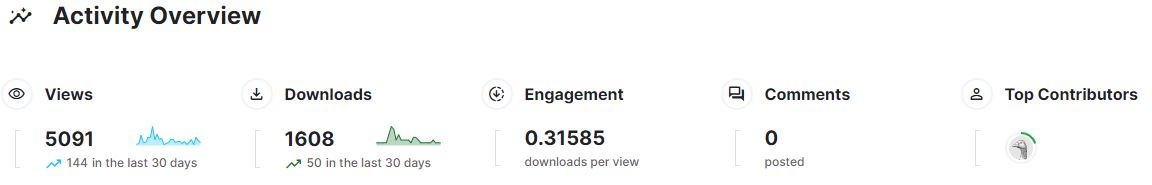
\includegraphics[width=\textwidth]{images/dataset/ds_1_activity.JPG}
    \caption{Activity Overview of the \emph{Climate Change Tweets} Dataset\protect\footnotemark}
    \label{fig:ds_1_activity}
\end{figure}
\footnotetext{Checked on May 9, 2024}

\paragraph{Dataset Advantages}
\begin{itemize}
    \item The dataset includes the text of each tweet along with its timestamp, providing a clear timeline of discussions.
    \item Metadata such as Likes, Retweets, and the number of comments are available, offering insights into the engagement each tweet received.
    \item The data is relatively recent, increasing its relevance to current studies on public opinion regarding climate change.
\end{itemize}

\paragraph{Dataset Disadvantages}
\begin{itemize}
    \item No sentiment scores are provided, requiring additional processing to analyze the sentiment of the tweets.
    \item The dataset covers only a seven-month period, limiting the ability to observe long-term trends or seasonal variations in the discussion of climate change.
    \item Accompanying the dataset is a single Jupyter notebook that contains minimal code unrelated to the dataset, offering little in terms of analysis or insights.
    \item There have been no updates to the dataset for two years, raising concerns about its currency and ongoing relevance.
\end{itemize}

\subsubsection{Climate Sentiment in Twitter}
The dataset Climate sentiment in twitter \cite{ClimateSentimentInTwitter} contains a single CSV file sized at 132.38 kB, containing 396 tweets with 14 columns, sourced from X between January 1, 2020, to December 24, 2020. It was gathered using the X API via the Tweepy library. Figure \ref{fig:ds_2_activity} shows that there is still user engagment, but not as active as for the previous dataset.

Key columns in the dataset include date, retweets, likes, text, location, and whether the user is verified. These columns offer valuable metadata about the timing, geographical context, and user engagement with each tweet.

\begin{figure}[h]
    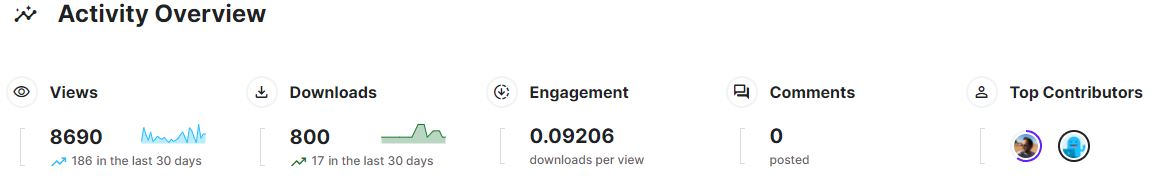
\includegraphics[width=\textwidth]{images/dataset/ds_2_activity.JPG}
    \caption{Activity Overview of the \emph{Climate sentiment in twitter} Dataset\protect\footnotemark}
    \label{fig:ds_2_activity}
\end{figure}
\footnotetext{Checked on May 10, 2024}

\paragraph{Dataset Advantages}
\begin{itemize}
    \item The dataset provides comprehensive metadata, particularly concerning time, location, and user interaction, which are crucial for detailed analyses.
    \item The methodology for data collection is documented, allowing for the potential expansion of the dataset using the specified Twitter API filters.
\end{itemize}

\paragraph{Dataset Disadvantages}
\begin{itemize}
    \item The overall description of the dataset is lacking, making it difficult to understand all aspects of the data without deeper investigation.
    \item It does not include sentiment scores, which would require additional processing to analyze the sentiment of the tweets
    \item The dataset is relatively small, covering only one year with an average of approximately 1.1 tweets per day covering only 1 year, which limits the scope of analysis.
    \item The data are somewhat outdated and not being updated anymore, which could affect the relevance and usefulness of the findings for current applications.
\end{itemize}

\subsubsection{Twitter Climate Change Sentiment Dataset}
The dataset Twitter Climate Change Sentiment Dataset \cite{TwitterClimateChangeSentimentDataset} provides a single CSV file of 6.57 MB, containing 43,943 tweets that have been annotated to reflect various sentiments toward climate change. These tweets are dated from April 27, 2015, to February 21, 2018, which was supported by a grant from the Canada Foundation for Innovation JELF, awarded to Chris Bauch at the University of Waterloo. The dataset includes three main columns: Sentiment, Message, and TweetID. The sentiment classes are detailed as follows:
\begin{itemize}
    \item \textbf{-1 (Anti):} The tweet expresses disbelief in man-made climate change.
    \item \textbf{ 0 (Neutral):} The tweet neither supports nor denies man-made climate change.
    \item \textbf{ 1 (Pro):} The tweet supports the belief in man-made climate change.
    \item \textbf{ 2 (News):} The tweet relays factual news about climate change.
\end{itemize}
Each tweet in the dataset was independently reviewed by three annotators for sentiment classification. A tweet was included in the final dataset only if there was unanimous agreement among all three reviewers regarding its sentiment class. The data were gathered using the X API within the specified date range. The methodology guarantee a comprehensive representation of public sentiment over the observed period.
Moreover, the dataset comes with detailed documentation that explains how the data was collected and labeled. Also, it includes nine notebooks created by different authors, filled with a lot of code to help with analyzing the data. Furthermore, this dataset has the most user attention of all datasets presented. Its activity overview can be found in figure \ref{fig:ds_3_activity}

\paragraph{Dataset Advantages}
\begin{itemize}
    \item The dataset is well-documented, providing clear insights into the data gathering and annotation processes.
    \item It is the largest dataset of its type currently developed, increasing its value for extensive research studies.
    \item The quality of the data is notably high, making it a reliable source for detailed analysis.
    \item High amount of existing code examples offer valuable resources for reuse and customizations, supporting further research and development. 
\end{itemize}
\paragraph{Dataset Disadvantages}
\begin{itemize}
    \item The dataset includes only 43,943 tweets, a modest number given the nearly three-year  timeframe of data collection, potentially limiting the scope of analysis.
    \item The data, covering dates up to early 2018, may not reflect current sentiments or recent developments in climate change discourse.
    \item There is no detailed explanation regarding the criteria used for selecting tweets for annotation, which might affect the dataset's applicability for certain research questions.
\end{itemize}

\begin{figure}[h]
    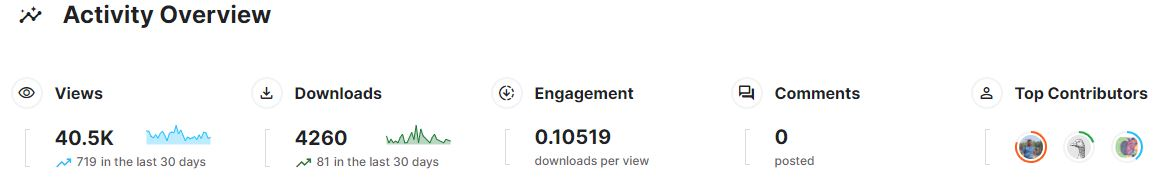
\includegraphics[width=\textwidth]{images/dataset/ds_3_activity.JPG}
    \caption{Activity Overview of the \emph{Twitter Climate Change Sentiment Dataset} Dataset\protect\footnotemark}
    \label{fig:ds_3_activity}
\end{figure}
\footnotetext{Checked on May 10, 2024}

\subsubsection{Social Media Sentiment and Climate Change}
The dataset Social Media Sentiment and Climate Change \cite{SocialMediaSentimentAndClimateChange} consists of six CSV files, with a combined size of 83.85 MB. The primary file in this dataset is the \emph{nltk\_split.csv} file. It includes important details such as the text of the posts, engagement metrics (favorite and retweet counts), the timestamp of posting, location coordinates, and an already calculated score for each post. Figure \ref{fig:ds_4_activity} shows its popularity.

\paragraph{Dataset Advantages}
\begin{itemize}
    \item Contains 164k posts.
    \item Provides a clear description on its Kaggle page.
    \item Covers about 20 months of data, from September 21, 2017, to May 19, 2019.
    \item Scores for posts are pre-calculated.
    \item Includes additional metadata for each post.
\end{itemize}

\paragraph{Dataset Disadvantages}
\begin{itemize}
    \item The methodology for score calculation is unknown.
    \item The latest entries are from mid-2019, making it around five years old.
    \item The specific social media platforms used for data collection are not identified.
    \item There appears to be redundancy among the data files.
    \item It is unclear whether "post" refers only to original content or also includes comments.
    \item There are no provided code examples to facilitate data analysis.
\end{itemize}

\begin{figure}[h]
    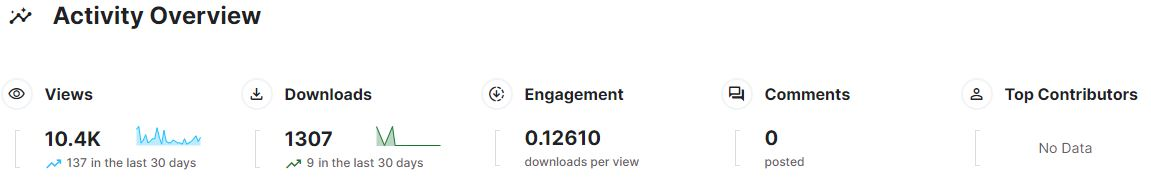
\includegraphics[width=\textwidth]{images/dataset/ds_4_activity.JPG}
    \caption{Activity Overview of the \emph{Social Media Sentiment and Climate Change} Dataset\protect\footnotemark}
    \label{fig:ds_4_activity}
\end{figure}
\footnotetext{Checked on May 11, 2024}

\subsubsection{The Reddit Climate Change Dataset}
The dataset The Reddit Climate Change Dataset \cite{TheRedditClimateChangeDataset} contains two CSV files obtained through \emph{SocialGrep Exports}, which collects all hits on \emph{climate} and \emph{change} that appear in the same comment (they don't necessarily need to appear as bigram): one file contains 620k posts and the other 4.6M comments, covering an extensive data range from January 1, 2010, to August 31, 2022, totaling about 12.5 years. The posts file includes 12 columns, with key columns being subreddit.name, created\_utc, and selftext. This file captures the important details of each post within the subreddit context. The comments file features 12 columns, notably created\_utc, body, and sentiment. This file provides insights into user interactions and sentiment across various discussions. Additionally, several code examples are provided to simplify data handling and analysis.
 
\begin{description}
    \item[SocialGrep Exports] is a feature offered by the SocialGrep tool \cite{SocialGrepExports}, which is designed to export and analyze data from social media platforms, notably Reddit. This feature enables users to download large datasets that include metrics such as post counts, engagement data, and sentiment analysis, all of which are useful for deep insights into social media trends and user behavior. The tool, SocialGrep, is owned and developed by Lexyr Inc., a company specializing in data analytics and extraction services. This makes SocialGrep an elemental part of Lexyr Inc.'s suite of tools that assist researchers, marketers, and analysts in using the power of big data from social media for various applications, from market research to academic studies.
\end{description}

\paragraph{Dataset Advantages}
\begin{itemize}
    \item Covers over 5 million posts and comments, offering a vast pool of social media interactions for analysis.
    \item Covers a considerable time period, including recent data up to August 2022.
    \item Pre-calculated scores for posts and comments are included, adding a layer of analysis readiness.
    \item Clear documentation of data sources improves the dataset's reliability.
    \item Availability of code examples benefits immediate data manipulation and analysis.
\end{itemize}

\paragraph{Dataset Disadvantages}
\begin{itemize}
    \item The description on Kaggle is not detailed, leaving several questions unanswered.
    \item A significant number of posts are inaccessible due to various restrictions like paywalls or provider limitations.
    \item Lack of clarity on how the scores for posts and comments were calculated.
    \item Both files include a 'score' column. However, the exact significance and calculation method of these scores are not fully explained.
    \item The large size of the files (262 MB and 4.11 GB) demands considerable computing resources and efficient programming to manage without exceeding system memory limits.
    \item There is no established linkage between posts and their corresponding comments, which complicates integrated analysis of conversations.
\end{itemize}

Despite its large data size, this dataset shows the highest engagement among all Kaggle datasets presented, as illustrated in Figure \ref{fig:ds_5_activity}.

\begin{figure}[h]
    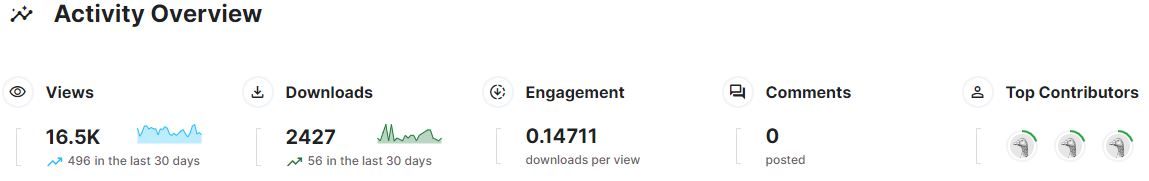
\includegraphics[width=\textwidth]{images/dataset/ds_5_activity.JPG}
    \caption{Activity Overview of the \emph{The Reddit Climate Change Dataset} Dataset\protect\footnotemark}
    \label{fig:ds_5_activity}
\end{figure}
\footnotetext{Checked on May 11, 2024}

\subsubsection{Final Dataset Selection}
\begin{table}[h!]
    \centering
    \begin{tabular}{c c c c c}
    \toprule
    \textbf{Dataset} & \makecell{\textbf{Number of} \\ \textbf{Comments}} & \makecell{\textbf{Level of} \\ \textbf{Documentation}} & \makecell{\textbf{Code} \\ \textbf{Availability}} & \makecell{\textbf{Sentiment} \\ \textbf{Availability}} \\
    \midrule
    \makecell{Climate Sentiment \\ in Twitter} & 396 & - & Yes & No \\
    \hline
    \makecell{Climate Change \\ Tweets} & 9,050 & - & No & No \\
    \hline
    \makecell{Twitter Climate \\ Sentiment Change \\ Dataset} & 43,943 & + & Yes & Yes \\
    \hline
    \makecell{Social Media \\ Sentiment and \\ Climate Change} & 164,000 & + & No & No \\
    \hline
    \makecell{The Reddit Climate \\ Change Dataset} & 4,600,698 & 0 & Yes & Yes \\
    \bottomrule
    \end{tabular}
    \caption{Datasets and their Key Properties for Dataset Selection}
    \label{table:datasets}
\end{table}

The dataset \emph{The Reddit Climate Change Dataset} is a great choice (see Table \ref{table:datasets} for a brief comparison) for studying how people feel about climate change because it covers a lot of ground and provides plenty of information. It covers a period of twelve years, which lets researchers see how opinions on climate change have changed due to major events, policy updates, and news coverage. With more than five million posts and comments, it covers a wide range of viewpoints, making sure that many different opinions are included.

The dataset also includes scores that hint at whether comments are positive, negative, or neutral towards climate change. These pre-calculated scores make it easier to quickly figure out the general mood in the data. Researchers can use these scores as a starting point to dive deeper into specific topics or time periods to understand how attitudes change.

Additionally, the dataset comes with some ready-to-use code, which makes it easier to start analyzing the data right away. This helps researchers focus on understanding the trends and patterns in how people talk about climate change, without getting pushed back by technical challenges. Overall, this dataset is very helpful for anyone looking to explore the complex ways people discuss and react to climate change over time.

\subsection{Reddit}
Reddit is one of the most popular social media platforms globally, especially noted for its appeal in English-speaking countries. Here, we provide a detailed breakdown of its demographics, language use, and popularity across different continents based on the latest data available.

\subsubsection{User Demographics and Global Reach}
\begin{description}
    \item[Geographical Distribution] As of 2023, the United States remains the dominant source of Reddit's traffic, accounting for approximately 47.89\% of all users. This high concentration highlights its significant impact on and usage by American audiences. Following the US, other significant traffic contributions come from:
    \begin{itemize}
        \item United Kingdom: 7.85\%
        \item Canada: 7.49\%
        \item Australia: 4.05\%
        \item Germany: 3.21\%
\end{itemize}
These figures underscore the platform's strong presence in predominantly English-speaking countries (Source: Alexa, 2023).

\item[User Age Group] The platform is particularly popular among younger demographics. Data from Statista (2023) indicate that:
\begin{itemize}
    \item 58\% of Reddit users are aged between 18 and 29 years.
    \item 29\% are aged between 30 and 49 years.
\end{itemize}
This demographic trend points to the platform's popularity among digital natives and younger internet users.

    \item[Gender Distribution] Approximately 70\% of Reddit users are male, which influences the type of content that is popular and the nature of discussions (Source: Statista, 2023).
\end{description}

\subsubsection{Language and Cultural Reach}
\begin{description}
    \item[Language Usage] While Reddit supports multilingual content, the predominant language of communication is English. This is reflected in the top countries by user base, all of which are primarily English-speaking nations. However, there are niche communities, known as subreddits, which meet specific languages and regional interests.
\end{description}

\subsubsection{Popularity Across Continents}
\begin{description}
    \item[North America and Europe] These regions represent the core user base of Reddit, with North America alone accounting for over half of all Reddit traffic. Europe, while having a diverse linguistic background, still contributes significantly to the user base due to the high English proficiency in countries like Germany, the UK, and the Nordic countries.
    \item[Asia and Other Regions] Reddit's presence in Asia is less pronounced, largely due to the prevalence of local social networks and language barriers. For instance, in China and South Korea, local platforms such as Weibo and Naver respectively, dominate the social media landscape. Reddit's market share in these regions is minimal.
    \item[Australia and Oceania] In Australia, Reddit enjoys considerable popularity, aligning with the global trend of English language dominance on the platform. The user engagement from this region is comparable to that of European countries.
\end{description}

\subsubsection{Conclusion}
These statistics provide a clear picture of Reddit's user base, highlighting its importance towards young, English-speaking populations primarily located in Western countries. This demographic and cultural profiling is crucial for understanding the context within which data from Reddit is generated and can be used in research to draw insights about Western, particularly American, public opinion and trends. Understanding these limitations is also vital for researchers using Reddit data to ensure that their findings are contextualized appropriately.

\section{Natural Language Processing Techniques}

\subsection{Sentiment Analysis and VADER}
\label{subsec:sentiment}
Sentiment analysis is a branch of natural language processing (NLP) that involves analyzing, understanding, and extracting opinions from text to determine the sentiment behind words. It is widely used to estimate public opinion, monitor brand and reputation, and understand customer emotions in text data.
\subsubsection{Toolkits for Sentiment Analysis}
There are several toolkits and libraries available for sentiment analysis, each offering unique features:
\begin{enumerate}
    \item \textbf{NLTK (Natural Language Toolkit):} This Python library is comprehensive for educational and research purposes, providing interfaces to over 50 corpora and lexical resources, including a built-in sentiment analysis module. It uses rule-based, lexicon-based methods for various NLP tasks \cite{BirdKleinLoper09}.
    \item \textbf{TextBlob:} Built on top of NLTK and Pattern, TextBlob is user-friendly for quick NLP tasks, offering a straightforward API for sentiment analysis. It provides a rule-based, lexicon-based API ideal for newcomers and intermediate users \cite{loria2018textblob}.
    \item \textbf{VADER (Valence Aware Dictionary and sEntiment Reasoner):} VADER is particularly tailored for social media analysis, employing a combination of qualitative and quantitative methods to determine sentiment. It excels in capturing the nuances of social media language, including emojis and slang. VADER uses lexicon-based methods with rule-based improvements \cite{hutto2014vader}.
    \item \textbf{spaCy:} Known for its speed and efficiency, spaCy supports sentiment analysis capabilities and is suitable for large-scale information extraction tasks, offering robust industrial-strength capabilities. spaCy is primarily automatic (machine learning), with support for rule-based extensions \cite{honnibal2017spacy}.
\end{enumerate}

\subsubsection{Approaches to Sentiment Analysis}
Sentiment analysis can be categorized into:
\begin{description}
    \item[Rule-Based Systems] Rule-based systems are tools which use specific grammar rules to figure out if words in a text are positive, negative, or neutral. They look closely at how sentences are built and pay attention to things like words that flip a meaning (like "not") or make it stronger or weaker. The great thing about these systems is that they're easy to understand. You can see how they work and even change the rules to suit your needs. This is really helpful when you need to explain why a piece of text was judged a certain way. However, these systems have some limitations. They can be hard to grow and adapt to new situations. It takes a lot of work to build and update them, especially when dealing with complicated texts or different languages and cultural settings. Also, they might not always get the sentiment right if the text has understated language keywords or cultural references that affect the meaning. This makes them less reliable in environments where language is constantly evolving or very diverse \cite{liu2012}.
    \item[Lexicon-Based Systems] Lexicon-based systems rely on a sentiment lexicon—a dictionary where each word is tagged with a predefined sentiment score. The overall sentiment of a text is calculated by summing the scores of the words present in the lexicon that appear in the text. This method is celebrated for its simplicity and efficiency, as it primarily involves dictionary lookups and arithmetic operations. However, its simplicity can also be a limitation. Lexicon-based systems typically do not account for the context surrounding words, which can lead to inaccuracies in texts where words may carry different sentiments depending on their usage. Moreover, these systems struggle with adaptability, often failing to recognize slang, idioms, or newly coined phrases that aren't included in the static lexicon. This makes lexicon-based sentiment analysis less reliable for texts that involve evolving language or colloquial expressions \cite{10.1162/COLI_a_00049}.
    \item[Automatic Systems] Automatic systems use machine learning algorithms to learn how to classify sentiment from large datasets of labeled text. These systems range from simpler models like logistic regression to more complex architectures such as deep learning models including Long Short-Term Memory (LSTM) networks or Convolutional Neural Networks (CNNs). One of the main advantages of automatic systems is their ability to understand complex language patterns and the context in which words are used, which significantly improves the accuracy of sentiment analysis across varied datasets. Additionally, these systems can adapt to new, unseen data if they are continuously trained, which is beneficial for applications involving dynamic language use. However, the dependency on large volumes of labeled training data makes these systems resource-intensive to develop. Furthermore, advanced models, particularly those based on deep learning, often lack interpretability, which can be problematic in settings where understanding the decision-making process behind sentiment analysis is essential \cite{yoonklim,pang2008opinion}.
    \item[Hybrid Systems] Hybrid systems represent an integration of rule-based, lexicon-based, and automatic methodologies, aiming to combine the strengths of each to optimize sentiment analysis. These systems might use machine learning models to analyze text structure and content, while rule-based adjustments are employed to refine the sentiment based on known linguistic cues. The flexibility and contextual relevance of hybrid systems are major advantages, as they allow for the integration of human insights through rules and tailored lexicons while using machine learning efficiencies. These systems often result in higher accuracy and robustness, particularly when dealing with specific linguistic or cultural distinctions. However, they can be complex to design and resource-intensive, requiring careful integration and significant computational power \cite{PORIA201650}.
\end{description}
These categories of sentiment analysis offer a spectrum of methodologies, each suited to different types of data and analysis needs. By understanding these distinctions, researchers and practitioners can better choose the approach that best fits their specific requirements for sentiment analysis.

\subsubsection{VADER and its Score}
VADER is specifically designed for sentiment analysis in social media contexts. Developed by Hutto and Gilbert (2014), VADER analyzes sentiments based on a lexicon of sentiment-related words and includes grammatical and syntactical rules to estimate textual sentiment. Its lexicon includes words that have been rated for their positive or negative sentiment valence based on common usage in social media environments. VADER is open-source, with its code and lexicon available on GitHub \url{https://github.com/cjhutto/vaderSentiment}, making it accessible for development and customization.

VADER outputs sentiment scores on a normalized, weighted composite scale. The compound score, which aggregates the cumulative sentiment of the text, ranges from -1 (extremely negative) to +1 (extremely positive). Scores are typically classified as follows:
\begin{itemize}
    \item \textbf{Positive sentiment:} compound score $\geq 0.05$
    \item \textbf{Neutral sentiment:} $-0.05 <$ compound score $< 0.05$
    \item \textbf{Negative sentiment:} compound score $\leq -0.05$
\end{itemize}
This scoring system allows for detailed interpretation of sentiment in text, particularly useful in dynamic and informal communication like social media posts. While VADER is highly effective for social media corpora, its performance can vary on more formal content or where context extends beyond the scope of its lexicon. Additionally, VADER may not always accurately interpret sarcasm, complex metaphors, or understated uses of language that may not directly trigger lexical keywords identified in its dictionary.

This detailed overview of sentiment analysis, particularly focusing on VADER, provides researchers and specialists with the necessary understanding to apply these methods effectively in different scenarios, especially where social media text analysis is required.

\subsection{Named Entity Recognition}
Named Entity Recognition (NER) is a process in natural language processing (NLP) where a computer reads a piece of text and highlights important names like people, companies, or places. This technology is crucial for understanding and organizing large amounts of data, as it helps convert unstructured text into structured data, making it easier to analyze.

\begin{description}
    \item[How NER Works] Imagine reading a news article. As you go through the article, you naturally pick out important names and details, such as the names of people involved, the places mentioned, or the dates of events. NER systems do something similar but in a more systematic way. For example, in the sentence "Microsoft announced a new product in Seattle", NER helps identify 'Microsoft' as a company and 'Seattle' as a location.
\end{description}

\subsubsection{Approaches to Sentiment Analysis}
\begin{enumerate}
    \item \textbf{Rule-Based Systems:} These systems use specific rules to find names. For example, a simple rule might be that any word starting with a capital letter after certain words like "in" or "at" is likely a place. These systems are straightforward and can be very accurate if the text is well-suited to the rules, but they can be too inflexible and might not work well with different kinds of text or languages.
    \item \textbf{Statistical Models:} These are more advanced systems that learn from examples. They look at large amounts of text to learn patterns about how names are used and can adjust to new information better than rule-based systems. They use techniques from statistics to predict whether a word or phrase is a name and what kind of name it is.
    \item \textbf{Deep Learning Approaches:} The newest and most advanced systems use deep learning, a type of AI that learns even more complex patterns from data. These systems, particularly ones using models like BERT from Google, are very good at understanding context, which helps them improve how they recognize names in sentences. They can learn from a broader range of examples and understand minor differences in how words are used.
\end{enumerate}

Advantages of NER are: 
\begin{itemize}
    \item \textbf{Fast and Efficient:} NER systems can quickly process lots of text, making them useful for handling large volumes of information.
    \item \textbf{Improves Data Quality:} By identifying and categorizing important names and details, NER helps make data easier to manage and analyze.
\end{itemize}

Disadvantages of NER are: 
\begin{itemize}
    \item \textbf{Struggles with Ambiguity:} Sometimes, NER systems get confused if a word has multiple meanings or uses, like "Apple" the company vs. "apple" the fruit.
    \item \textbf{Resource-Heavy:} The most advanced NER systems, especially those using deep learning, need a lot of computer power and data to learn effectively.
\end{itemize}

This explanation aims to make the concept of NER approachable and understandable, highlighting its key functions, the evolution of its techniques, and the practical challenges and benefits of its application in processing and analyzing text data.

\section{The Reddit Climate Change Dataset - Details, Data Selection and its Sentiment}
\label{section:datasetdetails}
In addition to the overview covered in section \ref{subsec:datasets}, this section investigates characteristics of the chosen dataset, including the data that will be used for following analysis. It also presents insights into the sentiment analysis provided, discussing its quality and origin methodology.

\subsubsection{Reddit Posts File}
As already described, the dataset contains two different CSV files. The file containing all available posts is named \emph{the-reddit-climate-change-dataset-posts.csv}. This file consists of approximately 620,000 entries, organized across 12 distinct columns that provide detailed information about each post:
\begin{itemize}
    \item \textbf{type:} This field identifies an entry as a "post" to differentiate it from comments.
    \item \textbf{id:} Each post has a unique identifier, for example, "x2nhvi".
    \item \textbf{subreddit.id:} This is a unique identifier for the subreddit, like "6wzx9b".
    \item \textbf{subreddit.name:} It shows the name of the subreddit, such as "advice".
    \item \textbf{subreddit.nsfw:} This boolean field indicates whether the post is considered not safe for work (NSFW)
    \item \textbf{created\_utc:} The date and time the post was created, given as a Unix timestamp.
    \item \textbf{permalink:} A permanent URL linking directly to the post.
    \item \textbf{domain:} The main web domain of the post's link, e.g., "twitter.com".
    \item \textbf{url:} Any external links included in the post.
    \item \textbf{selftext:} The text content of the post.
    \item \textbf{title:} The title of the post.
    \item \textbf{score:} The score of the post.
\end{itemize}
In this dataset, the "subreddit.nsfw" column shows that about 4,000 posts are labeled as NSFW, whereas the vast majority, 617,000, are not. The "created\_utc" timestamp is especially important for this thesis, as it helps track when each post was made, which is crucial for examining how discussions have evolved over time. This timestamp needs to be converted into a standard date and time format to make it more useful for analysis.

There is also a significant amount of missing data in the dataset. About 27\% of the entries in the "url" column are empty, indicating no external link was included. The "selftext" column, which should contain the main content of the posts, also frequently lacks useful information—with over 453,760 entries missing (marked as NaN), 52,800 deleted, and 71,799 removed. Interestingly, less than 7\% (effectively 42,549) of all entries contain actual text from the posts.

Also, the dataset includes a "score" column, which likely represents the net result of likes and dislikes for each post, effectively summarizing the overall community response. This column offers a straightforward metric to estimate the popularity or acceptance of the content within the platform.

Additionally, a complex and challenging feature of the dataset is that the "selftext" and "url" columns are never filled at the same time. The cause of this pattern is not immediately apparent, making it a potential topic for further exploration (not in scope of this thesis). This issue, combined with the widespread occurrence of incomplete or missing data, underscores the potential difficulties in using this dataset effectively.

\subsubsection{Reddit Comments File}
The file containing all available posts is \emph{the-reddit-climate-change-dataset-comments.csv}. This file consists of approximately 4.6m, organized across 10 distinct columns that provide detailed information about each comment. This file differs from the posts file in that it replaces columns such as \emph{domain}, \emph{url}, \emph{title}, and \emph{selftext}, but introduces two significant columns:
\begin{itemize}
    \item \textbf{body:} Contains the full text of each comment.
    \item \textbf{sentiment:} Represents the analyzed sentiment of the comment, with values ranging from -1 to 1, indicating the sentiment's polarity from negative to positive.
\end{itemize}
Notably, the Kaggle documentation does not explain how the sentiment values were derived, leaving the calculation method unclear. Additionally, the "body" column is consistently populated across all entries, ensuring that every comment in this file is usable for analysis.

\subsubsection{Data Selection}
In this thesis, the analysis will exclusively focus on the comments file rather than the posts file due to several advantages that improve the study's depth and reliability. Specifically, concentrating on the comments file is justified by the following points:
\begin{enumerate}
    \item \textbf{Richer Textual Content:} Comments often contain more direct and varied expressions of opinions as users engage with the content of the posts. This can provide deeper insights into public sentiment and reactions, which are crucial for understanding nuances in discussions related to complex topics like climate change.
    \item \textbf{Higher Engagement Metrics:} Comments can indicate higher engagement levels since they are responses to the posts. Analyzing comments can help understand which topics or aspects are driving more active discussions and debates among users.
    \item \textbf{Consistent Data Availability:} Every entry in the comments file has the 'body' field filled, ensuring that there is no missing textual data. This uniformity makes the comments file more reliable for comprehensive textual analysis, as it reduces the need to handle missing data.
    \item \textbf{Prepared for In-depth Sentiment Verification:} The comments file includes a 'sentiment' column, which provides initial sentiment scores for each comment. This setup is particularly useful as one of the initial tasks in this thesis involves analyzing and verifying these scores. Details of this verification process and the methodology applied will be discussed in the following sections of this thesis.
    \item \textbf{Broader Contextual Insights:} Since comments are reactions to posts, they often capture more dynamic and immediate responses to issues, offering broader insights into public opinion dynamics over time. This can be particularly useful in long-term studies where changes in public sentiment are analyzed.
\end{enumerate}
Focusing on the comments file will improve the efficiency and effectiveness of the analysis, especially when the research goal is centered around understanding detailed user interactions and sentiments rather than just the initial posts.

\subsubsection{Sentiment}
The origin of the sentiment scores provided in the dataset's "sentiment" column was initially unknown, initiating the first task of this thesis: to use the given sentiment values as a baseline and verify them by performing our own sentiment analysis. As detailed in section \ref{subsec:sentiment}, multiple approaches for sentiment analysis were considered, with VADER emerging as a suitable method due to its specialization in analyzing social media content.

Upon comparing the baseline sentiments from the dataset with those computed using VADER, it was determined that the provided sentiments correspond to the compound score generated by VADER. A slight discrepancy was noted: approximately 0.5 to 1.5\% of the scores per year are listed as NaN in the Kaggle dataset, whereas the VADER analysis consistently provided a numerical score. Examples of entries where Kaggle lists NaN but VADER provides a score include:
\begin{itemize}
    \item \emph{Climate Change WTF????} with a score of -0.4588,
    \item \emph{Climate change.} with a score of 0,
    \item \emph{Climate change :-)} with a score of 0.3182.
\end{itemize}
The reason why these sentiments match except for some entries being NaN remains unclear. However, moving forward, it is confirmed that the sentiment scores in the dataset can be reliably taken as VADER compound scores. All following sentiment-related investigations in this thesis will be based on this understanding, and no additional metrics will be introduced for comparison. The VADER score computed during this study is used, as the dataset had some NaN entries that required computation to ensure completeness and accuracy.

\chapter{Data Trends and Sentiment in Climate Change Discussions}
In this chapter, we explore the experimental design, results, and discussion of the study, focusing on the frequency distribution and sentiment analysis of Reddit comments related to climate change. The data source is "The Reddit Climate Change Dataset" which provides a comprehensive collection of comments from Reddit covering the years 2010 to 2022. We will explore how the volume of discussions and their sentiment have evolved over time, providing insights into public discourse on climate change.

\section{Frequency of Reddit Comments}
The first image (Figure \ref{fig:all_samples}) displays the absolute frequency of Reddit comments per year from 2010 to 2022. It is evident from the graph that there is a significant increase in the volume of comments over the years. Starting from a modest count in 2010, there is a sharp rise in 2019, peaking at 978,413 comments. This increase can be attributed to increased global awareness and discussions around climate change, fueled by significant events such as the Fridays for Future movement \cite{context2024greta,greenhouse2024greta} and the Australian bushfires \cite{wwf2024bushfires}. The years following 2019 show a slight decrease but remain significantly higher than the initial years. On average, the number of comments per year is 162,258 for Negative, 32,573 for Neutral, and 159,068 for Positive sentiments. The standard deviation for these classes is 151,771 for Negative, 31,635 for Neutral, and 143,654 for Positive sentiments, indicating considerable variability in the annual comment frequencies.
\begin{figure}[h]    
    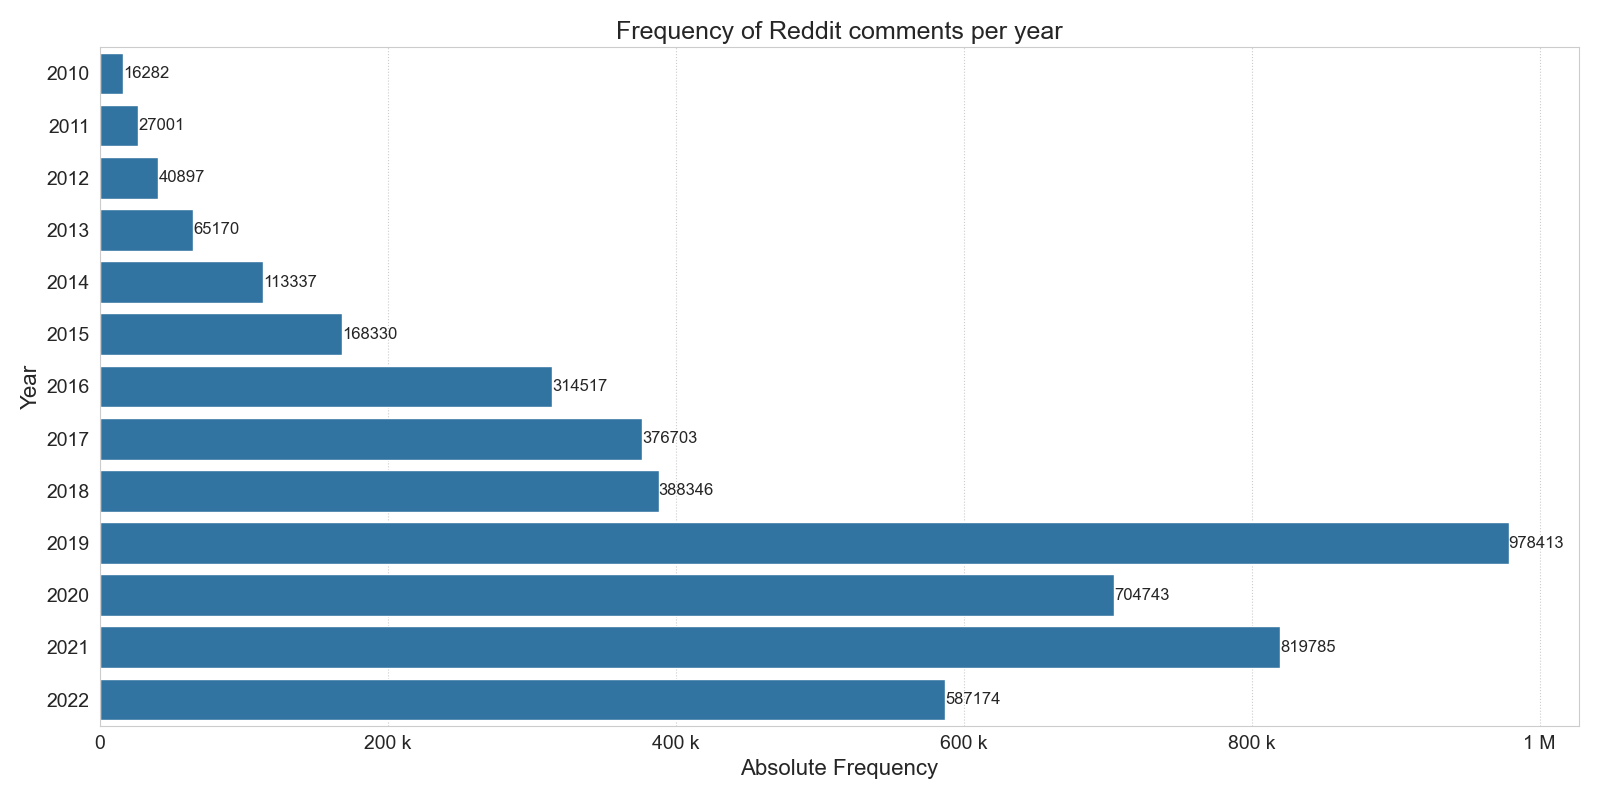
\includegraphics[width=\textwidth]{images/overview/samples_all.png}
    \caption{Distribution of Comments on Climate Change per Year}
    \label{fig:all_samples}
\end{figure}
This trend reflects the growing interest and concern among the public regarding climate change. The increase in comment frequency can be linked to major global events that brought climate issues to the forefront of public discourse. For example, the year 2019 saw a notable increase in comments, which coincides with widespread climate protests and significant media coverage of environmental issues \cite{euronews2023greta}.
The following image (Figure \ref{fig:all_samples_by_class}) breaks down these frequencies by sentiment class—positive, neutral, and negative—providing a more detailed view. Each bar is divided into three segments representing the proportion of each sentiment class. While the total volume of negative comments is higher overall, negative sentiment comments exceed positive ones in only four years: 2018, 2019, 2020, and 2022. This indicates that during these specific years, there were more discussions with a negative sentiment towards climate change topics among Reddit users. This could reflect increased awareness and concern about climate change impacts during those years, driven by specific events or developments. The year 2019 stands out with the highest number of negative comments, reflecting the heightened anxiety and negative sentiment during that period.
The dominance of negative sentiments suggests that climate change discussions on Reddit are often driven by worries and negative perceptions. This could be due to the alarming nature of news related to climate change, such as reports on natural disasters, policy failures, and scientific warnings about the impacts of climate change \cite{earthday2023climate}.
\begin{figure}[h]
    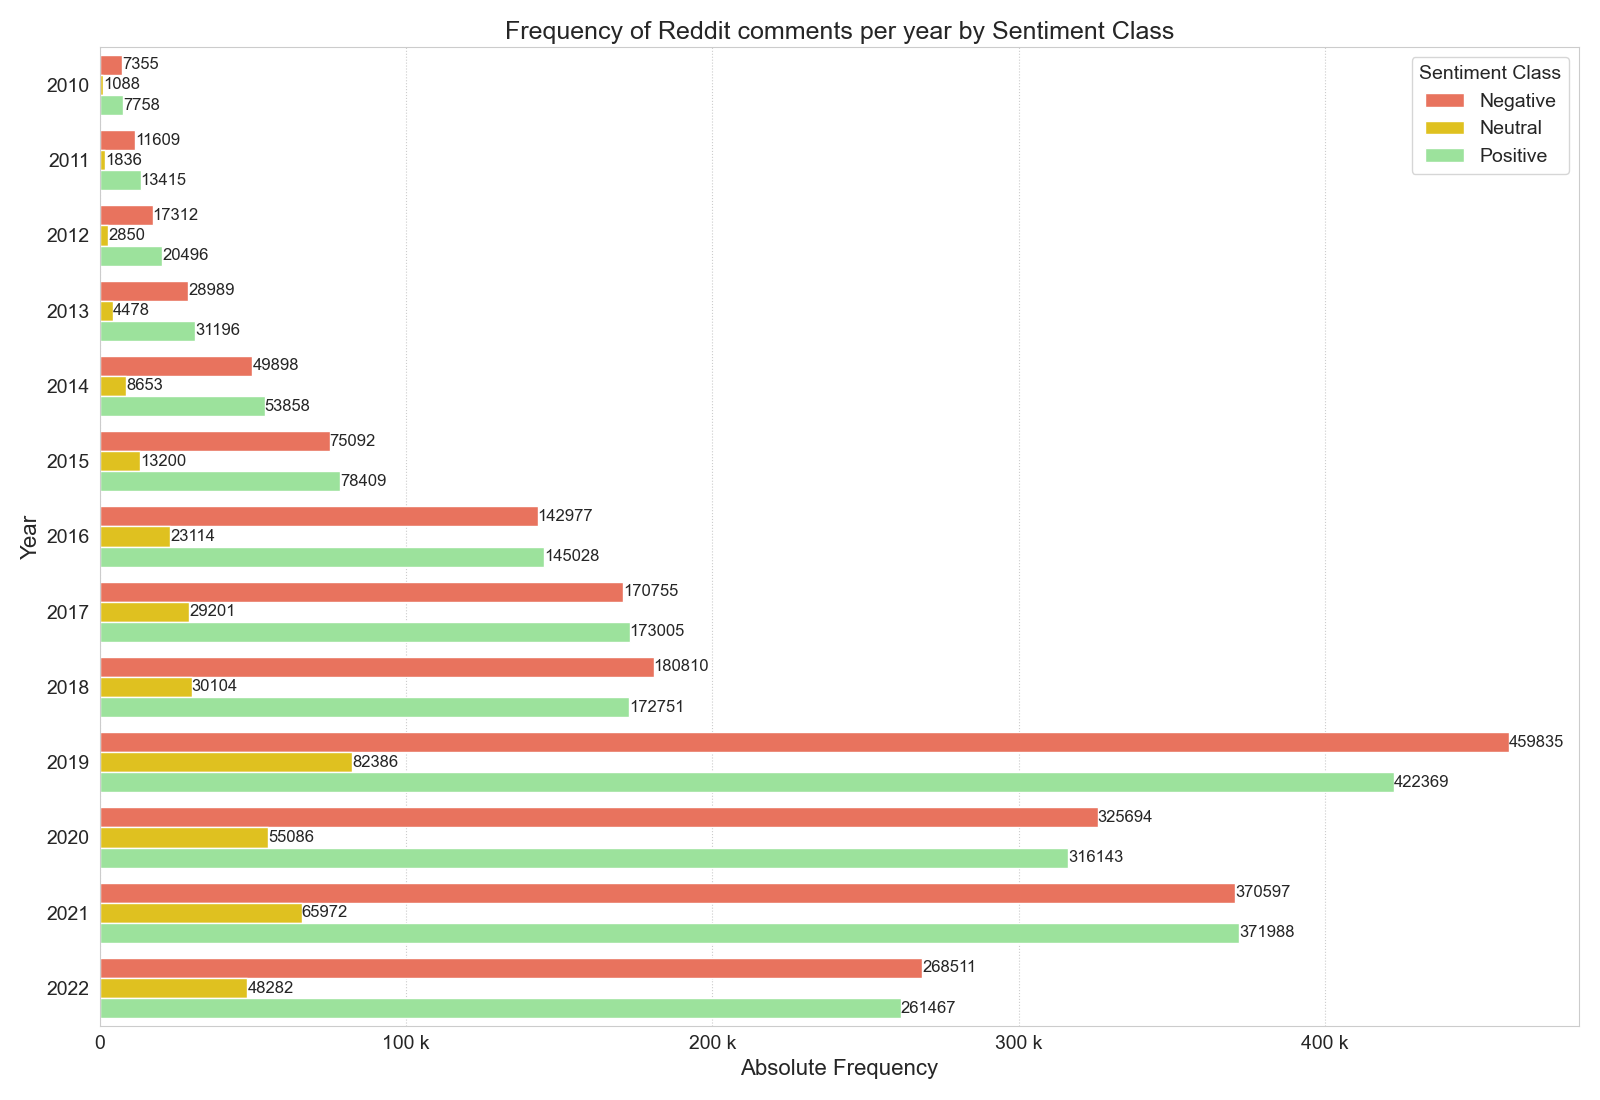
\includegraphics[width=\textwidth]{images/overview/samples_all_by_class.png}
    \caption{Distribution of Samples per Year by Sentiment Class}
    \label{fig:all_samples_by_class}
\end{figure}

\section{Distribution of Sentiment Classes}
\begin{figure}[h!]
    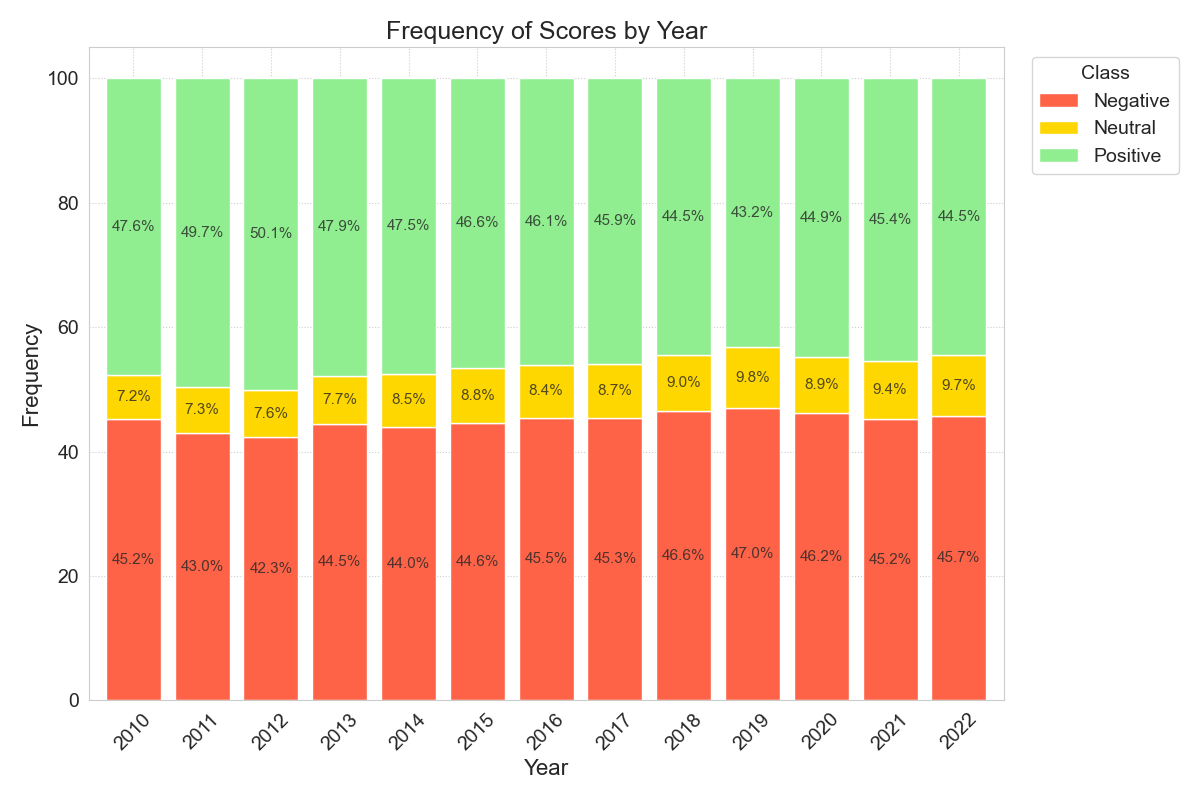
\includegraphics[width=\textwidth]{images/overview/samples_all_by_class_stacked.png}
    \caption{Percentage Distribution of Comments on Climate Change per Year by Sentiment Class}
    \label{fig:all_samples_by_class_percentage}
\end{figure}
In Figure \ref{fig:all_samples_by_class_percentage}, the percentage distribution of sentiment classes per year is presented. This stacked bar chart shows that while negative sentiments dominate the years 2018-2020 and 2022, there is a noticeable portion of positive and neutral sentiments as well. The proportion of neutral comments remains relatively stable, while positive comments show slight variations. The increase in negative sentiments around 2019 correlates with significant climate-related events that year, as previously mentioned. The data indicates that the public discourse on Reddit tends to be more critical or concerned regarding climate change.
Displaying both absolute numbers (Figure \ref{fig:all_samples_by_class}) and relative values (Figure \ref{fig:all_samples_by_class_percentage}) in sentiment analysis plots provides a comprehensive view of the data. The absolute numbers reveal the overall volume of comments, indicating trends in user engagement, while the relative values show the proportion of each sentiment class, highlighting shifts in sentiment distribution over time. This dual approach ensures a more detailed understanding of sentiment trends.
The persistent presence of negative sentiments highlights a continuous public concern about climate change. Neutral comments, which make up a considerable portion, likely include factual statements and information sharing, indicating that many users are discussing climate change in an informative manner. The slight variations in positive comments suggest occasional optimism, possibly related to breakthroughs in climate science, successful environmental policies, or inspiring activism.

\section{Mean Sentiment Over Time}
The image in Figure \ref{fig:mean_sentiment} plots the mean VADER sentiment score per year, providing an overview of the general sentiment trend. The sentiment scores fluctuate over the years, with notable peaks and drops corresponding to significant climate-related events. For instance, the negative decrease around 2018 aligns with the intense climate protests and global movements that provoked widespread discussions and emotional responses. Overall, the sentiment trend illustrates the evolving public sentiment towards climate change, marked by periods of optimism and concern.
The mean sentiment score reveals the general mood of the public regarding climate change over time. The positive peaks might correlate with successful climate initiatives or positive media coverage, while the negative drops reflect times of crisis or heightened awareness of climate issues. This trend underscores the impact of global events and media coverage on public sentiment, highlighting the dynamic nature of climate change discourse on social media \cite{Valentini2016}.

A significant factor influencing these discussions is the role of influential climate activists such as Greta Thunberg. Greta Thunberg, a Swedish environmental activist, gained international recognition for her efforts to tackle climate change. Her Fridays for Future movement, which began as a solo protest outside the Swedish parliament, inspired millions of young people around the world to participate in climate strikes \cite{fridaysforfuture2024ruckblick}. Thunberg's speeches at major international forums, including the United Nations \cite{un2019greta}, have inspired public opinion and brought the urgency of climate action to the forefront of global discourse (Jones, 2021).
Thunberg's activism, particularly around 2018 and 2019, contributed to the surge in climate-related discussions on Reddit. Her ability to express the fears and hopes of a younger generation has had a significant impact on many, driving both positive and negative sentiments in online discussions. The increase in negative sentiments during these years can be partly attributed to the polarized reactions to her outspoken stance on climate issues \cite{aidr2024blacksummer}.

This detailed examination provides a comprehensive overview of the dynamics of climate change discourse on Reddit, highlighting the patterns of public sentiment and the influence of significant global events and prominent activists. The data underscores the complex interplay between public opinion, media coverage, and impactful events in shaping the conversation around climate change.

\begin{figure}    
    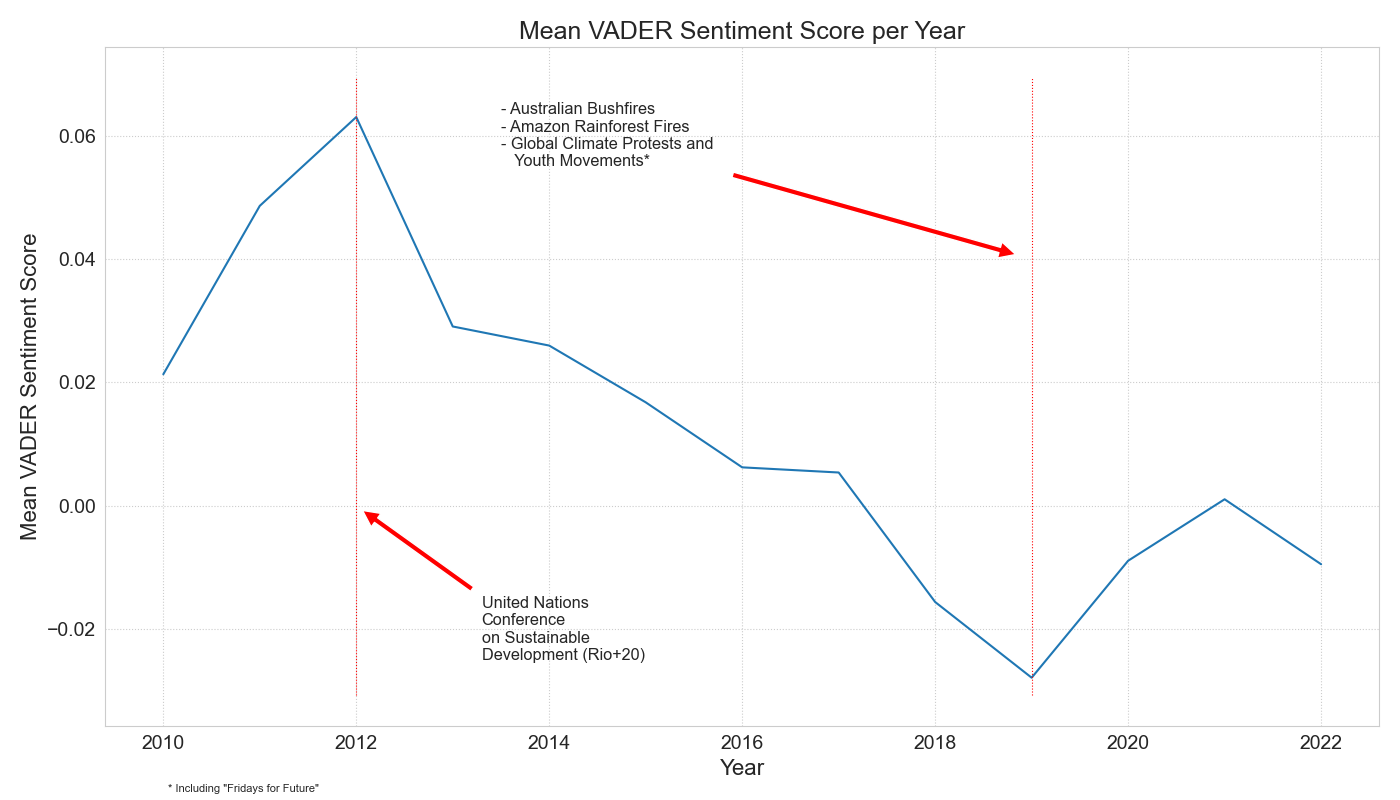
\includegraphics[width=\textwidth]{images/overview/mean_sentiment.png}
    \caption{Annual Average Sentiment with Event Highlighting}
    \label{fig:mean_sentiment}
\end{figure}

\section{Top 5 Frequent Subreddits}
\begin{figure}
    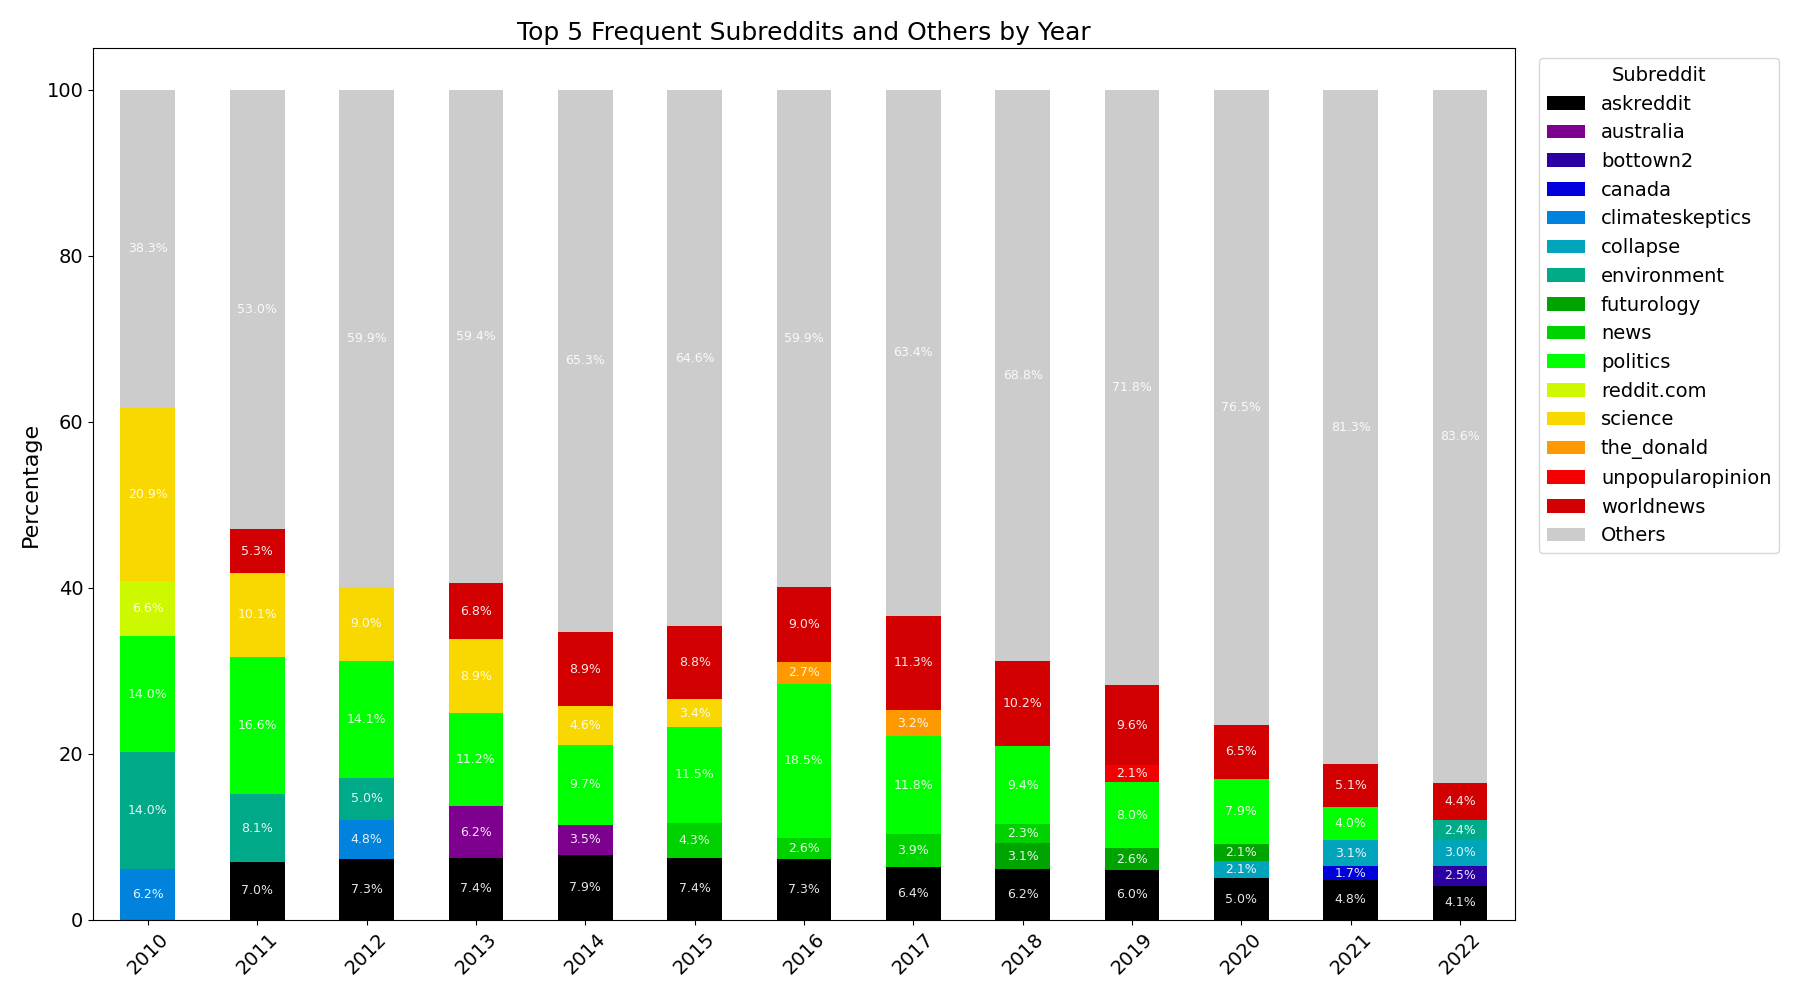
\includegraphics[width=\textwidth]{images/overview/subreddit_frequency_top5.png}
    \caption{Yearly Top Five Subreddits and their Percentual Relation}
    \label{fig:top5subreddits}
\end{figure}
Figure \ref{fig:top5subreddits} illustrates the five most frequent subreddits by year, alongside a category labeled \emph{Others}. This graph provides insight into which subreddits are most active in discussions about climate change. The \emph{Others} category covers all subreddits that are not within the top five for a given year, highlighting the contributions of a broad range of subreddits to the climate change discourse. The dominance of \emph{Others} suggests that climate change is a topic of widespread interest across many different communities on Reddit, indicating that it becomes more relevant to more areas of our life and conversations. Specific subreddits such as \emph{worldnews}, \emph{science}, and \emph{politics} are consistently among the top contributors, reflecting the intersection of climate change with global events, scientific discussion, and political debate.

The diverse range of subreddits involved in climate change discussions, as indicated by the significant \emph{Others} category, suggests that the topic spreads through various aspects of society, from politics and science to general news and public opinion \cite{doi:10.1177/1329878X211038004}. The presence of subreddits like \emph{the\_donald} and \emph{unpopularopinion} in certain years indicates that climate change is also a point of debate and differing viewpoints. The fluctuation in subreddit participation over the years can reflect shifts in public interest and the emergence of new influential communities on Reddit.

\section{Comment Length Analysis}
\begin{figure}[h]
    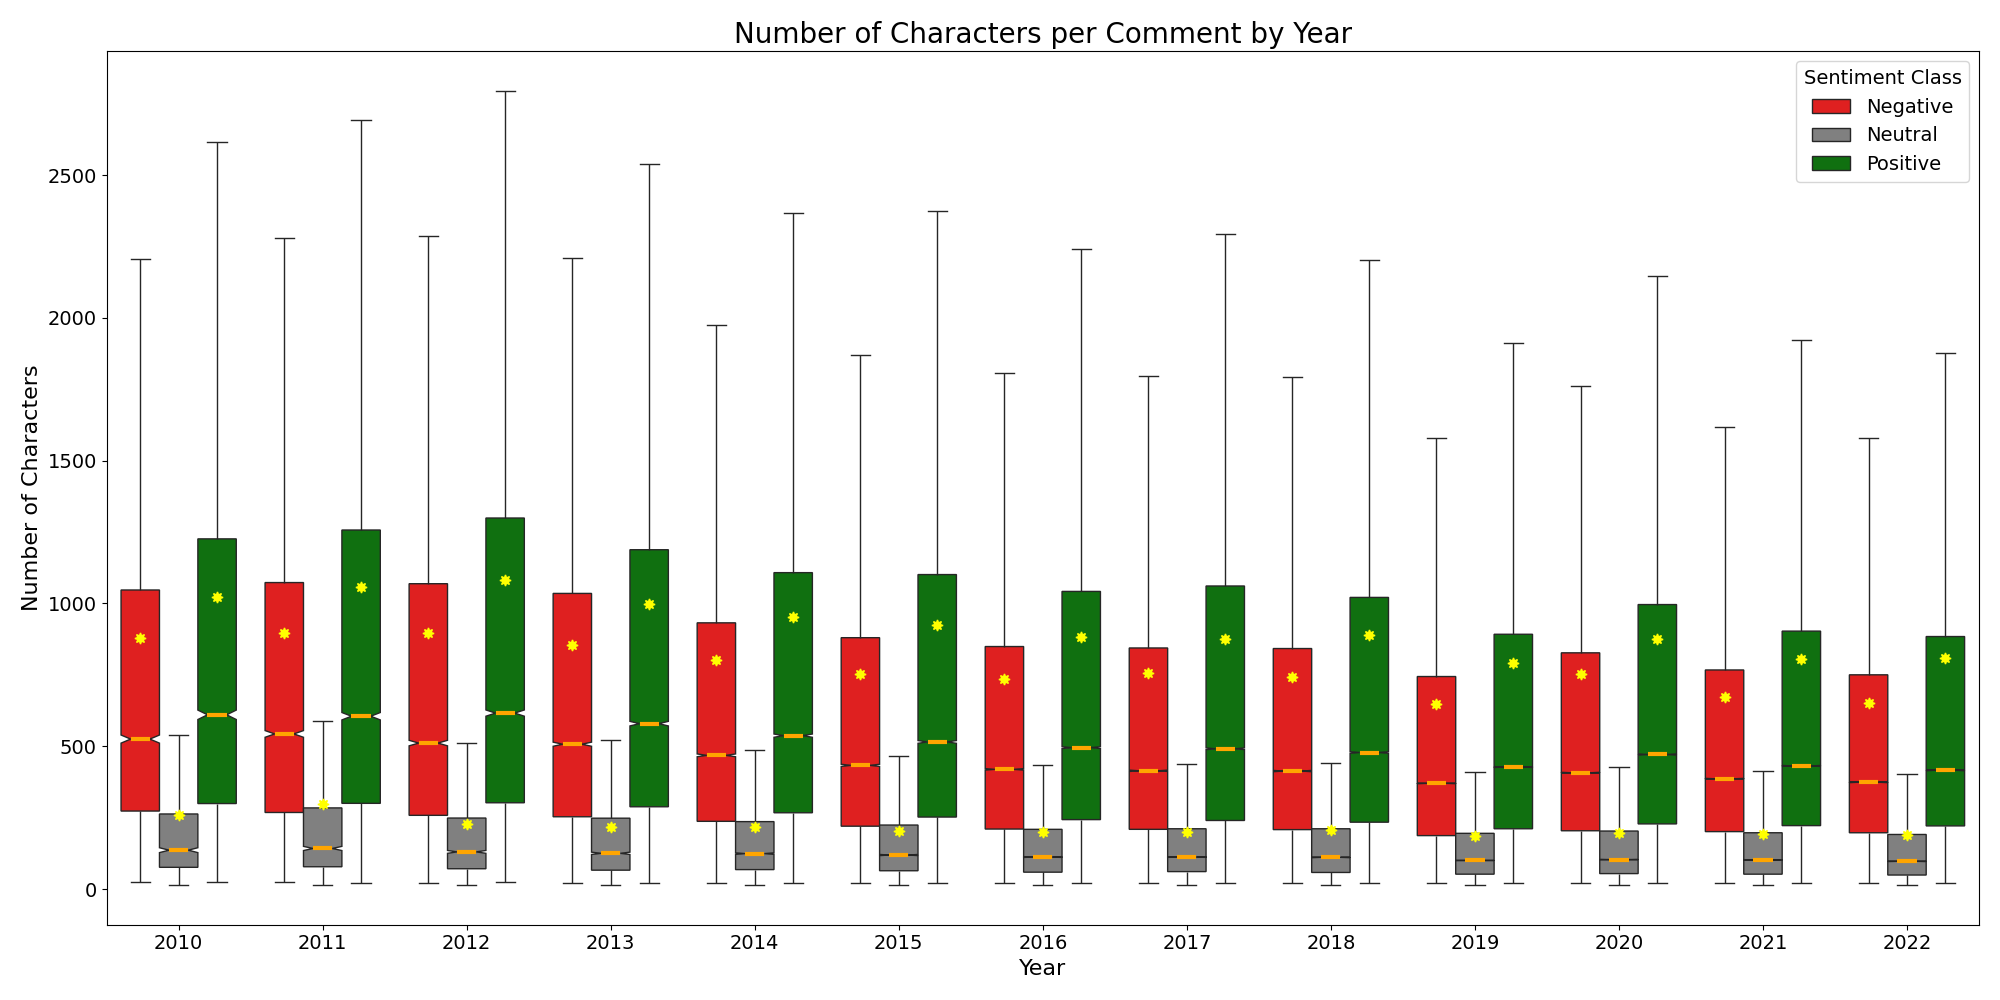
\includegraphics[width=\textwidth]{images/overview/comment_length_boxplot.png}
    \caption{Boxplot of the Comment Length by Sentiment Class}
    \label{fig:boxplot_comment_length}
\end{figure}
Figure \ref{fig:boxplot_comment_length} displays a boxplot of the number of characters per comment by year, segmented by sentiment class. This analysis reveals that comments with positive sentiments tend to be longer compared to those with negative or neutral sentiments. The longer length of positive comments indicates that these discussions are often more detailed and elaborate. On average, the length of negative comments is 706.76 characters with a standard deviation of 984.78, neutral comments average 195.46 characters with a standard deviation of 382.73, and positive comments average 848.30 characters with a standard deviation of 1177.78. This indicates a considerable variability in comment lengths, particularly for positive comments.
Longer comments usually show more detailed discussions. The data shows that users tend to write more extensively when expressing positive sentiments, possibly to share their support for climate initiatives or detailed success stories. These positive comments help build a supportive environment and promote constructive discussions about climate change solutions. Negative comments, while generally shorter, might still reflect strong emotions such as frustration or anger, leading users to provide critiques or express their feelings. Neutral comments are typically the shortest, focusing on sharing straightforward information without much additional commentary \cite{orglearning}.
Understanding these patterns is important for several reasons. First, the depth of engagement in positive comments suggests that users who are optimistic about climate change solutions are more likely to share detailed information and experiences. This can enrich the conversation and provide valuable insights for others. Recognizing the potential for detailed negative comments driven by frustration can help ensure that these contributions remain constructive and do not escalate tensions.

In conclusion, this confirms that positive comments on climate change tend to be more detailed and longer compared to negative and neutral comments. This trend is constant across all the years analyzed, indicating that positive discussions involve more complex and extensive commentary. Understanding these patterns is crucial for promoting meaningful conversations about climate change and ensuring a balanced discourse that includes both emotional and factual content.

\chapter{Analysis of Specific Topics in Climate Change Discussions}
\section{Key Terms (N-grams) and their Frequency \& Sentiment}
In this section, the trends in climate change discussions on Reddit are explored by analyzing the frequency and sentiment of key terms over time. Using the \emph{Counter} class from Python's \emph{collections} module, the most frequently mentioned unigrams and bigrams related to climate change were identified. Initially, the most frequent 100 uni- and bigrams were calculated. However, due to the non-preprocessed nature of the dataset, many of these frequent terms did not offer much meaningful information (e.g., terms like "http", "just", "know", "like", "make need", "don think", "don believe", "org wiki", "feel like"). Therefore, several relevant terms were manually hand-picked to focus on in the analysis. This approach provides clearer insights into the shifting focus of climate-related conversations and the associated sentiments expressed by Reddit users.

\subsection{Unigrams}
\subsubsection{Frequency}
\begin{figure}[h]
    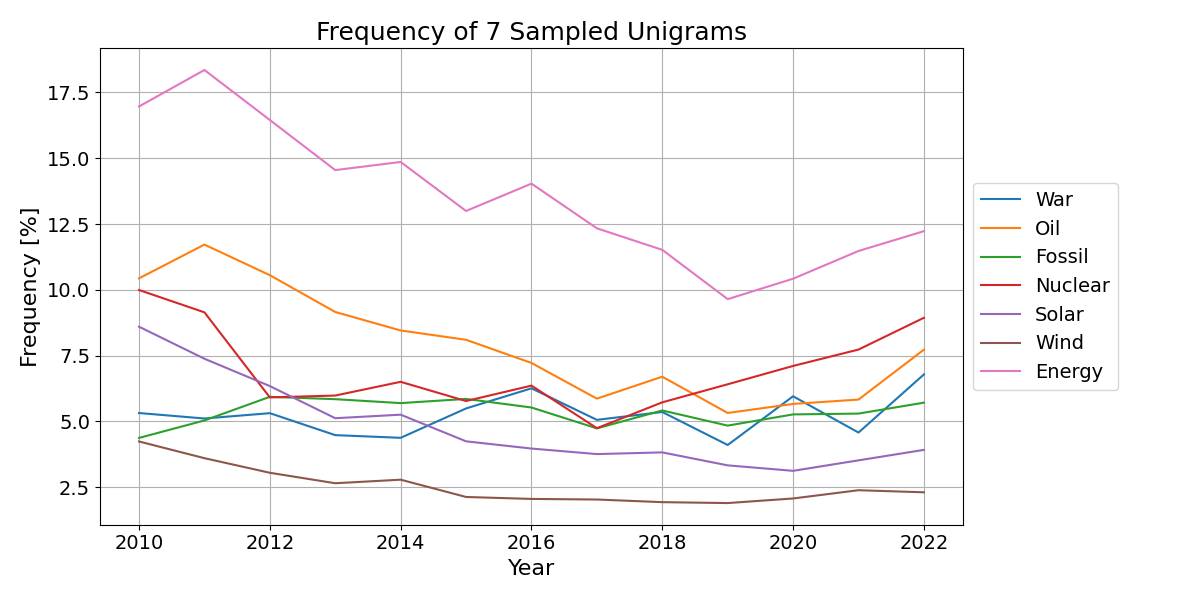
\includegraphics[width=\textwidth]{images/topic_details/ngram/frequency_per_topic_7Unigram.png}
    \caption{Frequency distribution of unigrams war, oil, fossil, nuclear, solar, wind, and energy}
    \label{fig:frequency_unigrams}
\end{figure}
The plot in Figure \ref{fig:frequency_unigrams} presents the frequency of seven selected unigrams over time. These unigrams include "war", "oil", "fossil", "nuclear", "solar", "wind", and "energy". The frequency is represented as a percentage of total unigram occurrences per year. The selected key terms, except for \emph{war}, are all related to energy. Energy is a crucial factor in the context of climate change because the production and consumption of energy are major sources of greenhouse gas emissions. Changing to renewable energy sources like solar and wind, and reducing dependence on fossil fuels such as oil and nuclear energy, are essential strategies for mitigating climate change and achieving sustainable development. These energy-related discussions reflect the importance of energy policy and technology in addressing climate change challenges.

The term \emph{war} is included in the analysis to highlight its relevance to climate change discussions especially when it comes to its sentiment. Conflicts and geopolitical tensions can have significant impacts on energy resources and climate policies, making it an important topic within the broader context of climate change discourse. Also, this indicates that discussions about war and its impact on climate change have been a consistent topic of interest. Debates about the environmental impacts of wars, such as resource consumption and destruction of ecosystems, contribute to this trend \cite{hsiang2014climate}.

Both \emph{oil} and \emph{fossil} terms show different trends. The frequency of discussions around \emph{oil} shows a decrease over the years, reflecting a growing awareness and shift towards renewable energy sources and away from fossil fuels. On the other hand, the term \emph{fossil}, represented by the green line, remains relatively stable with a slight increase. This stability and slight increase might indicate ongoing discussions about fossil fuels, especially in the context of debates around energy policies and climate change mitigation strategies. Major events, such as the Paris Agreement in 2015, which aimed to limit global warming by reducing greenhouse gas emissions, played a significant role in shifting public and policy focus towards cleaner energy alternatives \cite{unfccc2015paris}.

The frequency of \emph{nuclear} discussions has a noticeable drop post-2011, aligning with the Fukushima Daiichi nuclear disaster. This incident raised global concerns about the safety of nuclear energy, leading to more cautious and often negative discussions around this energy source \cite{WNA2012}. The decrease is also associated with several countries re-evaluating their nuclear policies and energy strategies as a result of the disaster.

\begin{figure}[h]
    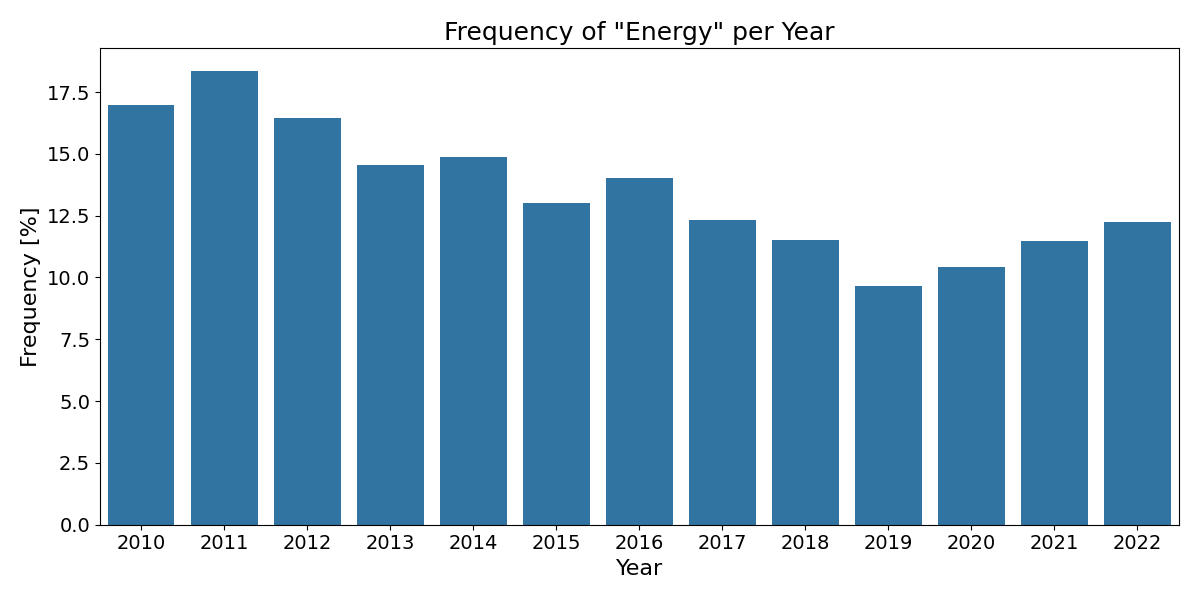
\includegraphics[width=\textwidth]{images/topic_details/ngram/frequency_bar_energy.png}
    \caption{Detailed Frequency Distribution of \emph{energy}}
    \label{fig:frequency_energy}
\end{figure}

Terms like \emph{solar} and \emph{wind} show a decreasing trend over the years. The frequency of discussions around \emph{wind} energy, represented by the brown line, has decreased from approximately 4\% to 2.5\%. Similarly, the frequency of \emph{solar} energy discussions, represented by the purple line, has dropped from around 9\% to 4\%. This decreasing trend could be attributed to the initial rise in discussions and interest when these technologies were newer and perceived as more revolutionary. As these renewable energy sources have become more established and integrated into mainstream energy discussions, the novelty may have worn off, leading to fewer mentions relative to other topics. However, the ongoing interest and investment in renewable energy technologies are driven by government policies and international commitments to reduce greenhouse gas emissions, such as the European Union's Renewable Energy Directive and various national incentives for renewable energy projects \cite{irena2018roadmap}.

The term \emph{energy} with a detailed bar plot in Figure \ref{fig:frequency_energy} shows the frequency of the term \emph{energy} per year. The term has been consistently discussed, with a notable peak in 2011. This rise likely corresponds to increased discourse surrounding energy policies and the push for sustainable energy solutions during that period. The global focus on energy efficiency and the transition to renewable energy sources could have driven these discussions. The increased focus on energy in 2011 may also be attributed to policy discussions and implementations following the Fukushima disaster, emphasizing the need for safer and cleaner energy alternatives \cite{iea2011policies}.

\subsubsection{Sentiment}
\begin{figure}[h]
    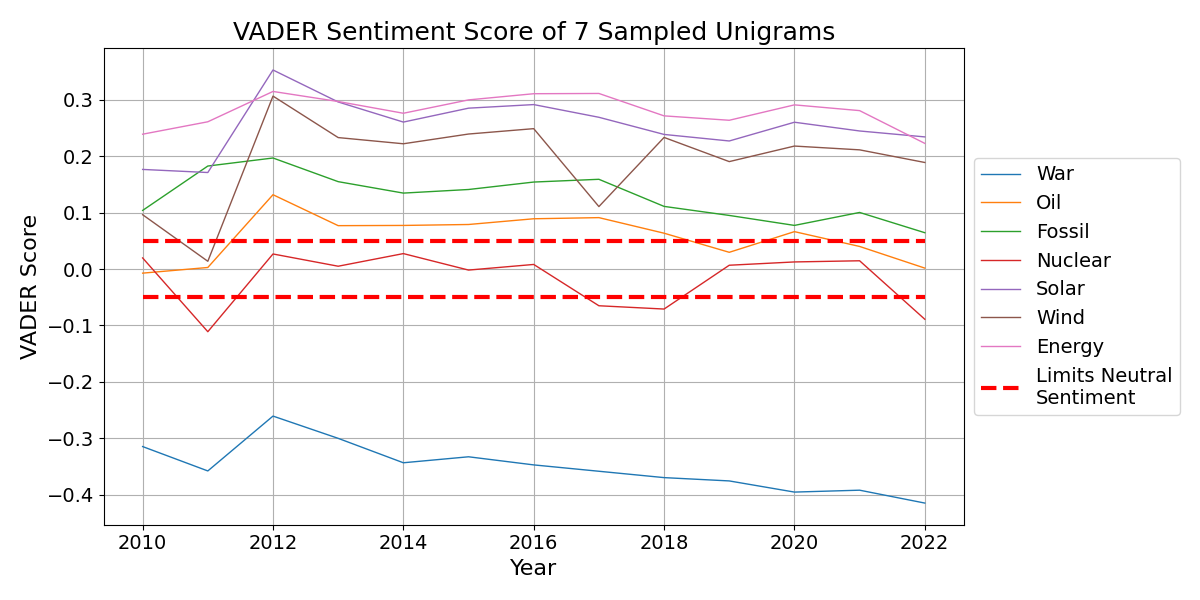
\includegraphics[width=\textwidth]{images/topic_details/ngram/sentiment_per_topic_7Unigram.png}
    \caption{Sentiment Scores of Unigrams \emph{war}, \emph{oil}, \emph{fossil}, \emph{nuclear}, \emph{solar}, \emph{wind} and \emph{energy}}
    \label{fig:sentiment_unigrams}
\end{figure}
The sentiment plot in Figure \ref{fig:sentiment_unigrams} displays the VADER sentiment scores for the same set of unigrams. Sentiment scores range from -1 (very negative) to 1 (very positive), with the red dashed lines indicating the limits for neutral sentiment.

\emph{War} consistently holds a negative sentiment, reflecting the unfavorable impacts and concerns associated with war on the environment and society. On the other hand, \emph{energy} shows the highest positive sentiment overall, indicating optimistic discussions about energy solutions and innovations. The positive sentiment around \emph{energy} suggests that discussions are often framed in a constructive context, focusing on advancements and potential solutions for climate change.

\emph{Nuclear} experiences its lowest sentiment in 2011, reflecting public doubts about nuclear energy's safety and environmental risks. This is a direct consequence of the Fukushima disaster, which led to a rise in negative perceptions about nuclear energy globally \cite{WNA2012}. Despite this, \emph{nuclear} sentiment scores are generally within the neutral range, except for the drops in 2011, 2017, 2018, and 2022. The relatively neutral sentiment in other years suggests that discussions about nuclear energy include both its risks and its potential as a low-carbon energy source.

Conversely, \emph{solar} and \emph{wind} maintain generally positive sentiments, highlighting favorable perceptions and the potential of these renewable energy sources in mitigating climate change. This positive outlook is likely driven by the increasing efficiency, decreasing costs, and widespread adoption of solar and wind technologies \cite{irena2018roadmap}. Even \emph{oil} despite its association with fossil fuels, shows a positive sentiment in most years, reflecting discussions around technological advancements in reducing emissions or the economic importance of oil.

Several factors could contribute to \emph{oil} maintaining a higher sentiment than \emph{nuclear}. First, oil has historically been a critical driver of economic growth, providing energy for transportation, industry, and households \cite{CAVALCANTI2013475}. Discussions about oil often highlight its economic benefits and the technological advancements aimed at reducing its environmental impact, such as carbon capture and storage (CCS) and cleaner extraction methods (IEA, 2019).
Second, the oil industry has invested significantly in public relations and marketing to maintain a positive image, emphasizing the role of oil in modern society and efforts to transition to cleaner technologies \cite{ExxonMobil2021}. This could lead to a more favorable perception of oil compared to nuclear energy, which has struggled with public relations, particularly after high-profile accidents like Chernobyl and Fukushima.
Overall, while \emph{nuclear} energy is perceived neutrally to negatively, \emph{oil} consistently maintains a higher sentiment, except for 2010. This trend might be due to ongoing discussions about the economic benefits of oil and advancements in cleaner technologies for its use, which can sometimes overshadow the negative aspects related to its environmental impact.

\subsection{Bigrams}
\subsubsection{Frequency}
\begin{figure}[h]
    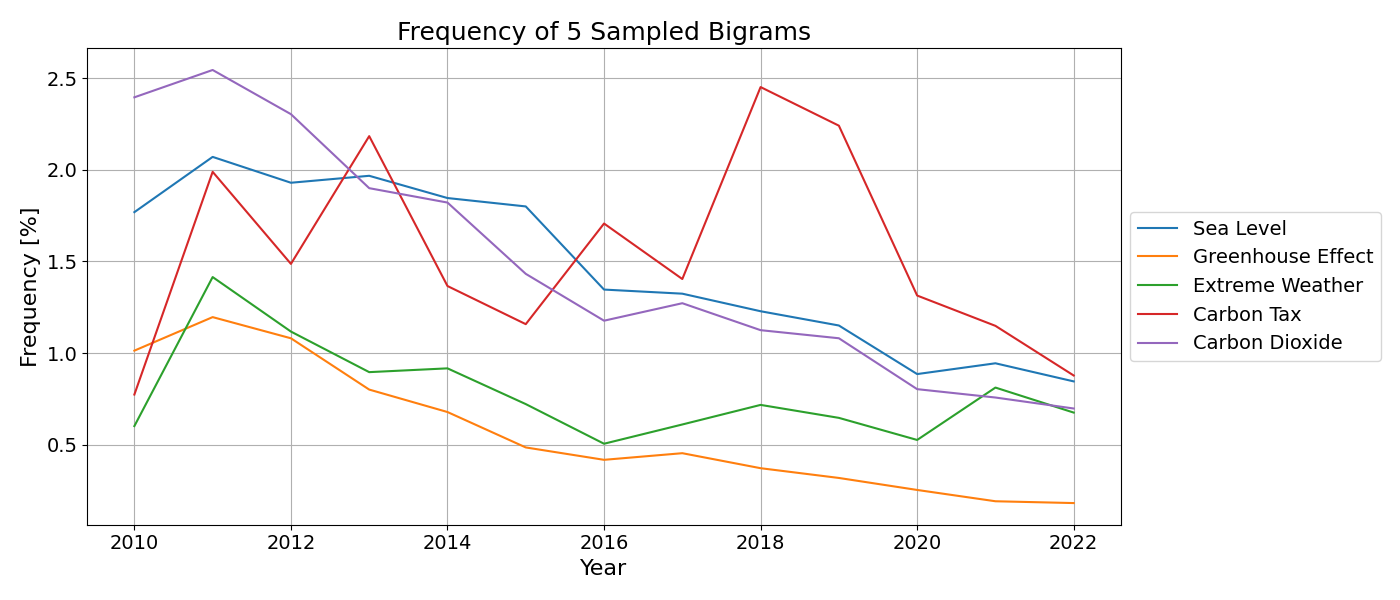
\includegraphics[width=\textwidth]{images/topic_details/ngram/frequency_per_topic_5Bigram.png}
    \caption{Frequency Distribution of Bigrams \emph{sea level}, \emph{greenhouse effect}, \emph{extreme weather}, \emph{carbon tax} and \emph{carbon dioxide}}
    \label{fig:frequency_bigrams}
\end{figure}

The plot shown in Figure \ref{fig:frequency_bigrams} provides the frequency of five selected bigrams: sea level, greenhouse effect, \emph{extreme weather}, carbon tax and \emph{carbon dioxide}

The term \emph{carbon tax} peaks in frequency in 2011, 2013, 2018, and 2019. These peaks correspond to periods of intense policy discussions and implementations related to carbon pricing mechanisms. For example, in 2011, Australia introduced a significant carbon tax aimed at reducing carbon emissions, leading to extensive debates and discussions \cite{worldbank2018carbon}. In 2013, British Columbia's carbon tax was widely discussed due to its innovative approach and effectiveness in reducing emissions \cite{murray2015bc}. The peaks in 2018 and 2019 align with renewed global discussions on carbon pricing as a critical tool for meeting the Paris Agreement targets, with several countries either implementing or considering carbon tax policies during these years \cite{worldbank2018carbon}.
The term \emph{carbon tax} also highlights the complexities and challenges associated with implementing such policies. These discussions often center around economic impacts, public acceptance, and the effectiveness of carbon taxes in reducing emissions. The repeated peaks suggest that the topic remains disputed and relevant, reflecting ongoing policy evaluations and adjustments in various regions. The fluctuation in frequency underscores the dynamic nature of climate policy debates and the role of public discourse in shaping these policies.

The decreasing trend of \emph{greenhouse effect} suggests that the term may be getting replaced by more specific and complex discussions around climate change impacts and solutions. This could reflect a shift in discourse from basic concepts to more complex and targeted climate change issues, such as carbon footprints, renewable energy technologies, and specific environmental policies \cite{ipcc2014impacts}. The decreasing use of \emph{greenhouse effect} may indicate that the public and policymakers are moving beyond basic education about climate change to more action-oriented discussions.
Furthermore, the reduction in the use of \emph{greenhouse effect} might also be attributed to the evolution of climate change communication strategies. As public understanding of climate change has increased, there has been a corresponding shift towards discussing mitigation and adaptation strategies in more specific terms. This shift is essential for driving effective policy measures and encouraging practical solutions to tackle climate change. It also reflects the broader trend in environmental communication, where the focus is increasingly on actionable steps rather than basic concepts.

Another significant observation is the decrease in the frequency of \emph{sea level} and \emph{carbon dioxide}. The frequency of \emph{sea level} discussions has significantly dropped over the years. This might be due to the increasing focus on more immediate and impactful climate issues such as renewable energy sources and policy measures like carbon taxes. Although sea level rise remains a critical aspect of climate change, the public discourse may have shifted towards addressing the causes of climate change more directly, such as carbon emissions and energy use \cite{nasa2020,nasa2020co2}.

The term \emph{carbon dioxide} shows a noticeable decrease in frequency, dropping from approximately 2.4\% to 0.7\%. This drop could indicate a shift in the language used to discuss emissions and climate change. As climate science and policy discussions have evolved, terms like \emph{carbon footprint} or \emph{greenhouse gases} might be more frequently used, reflecting a broader understanding and more sophisticated discourse about emissions and their impacts \cite{unep2019}. The shift from \emph{carbon dioxide} to other terms might also suggest a more integrated approach to discussing various greenhouse gases collectively, rather than focusing on a single component.

\subsubsection{Sentiment}
\begin{figure}[h]
    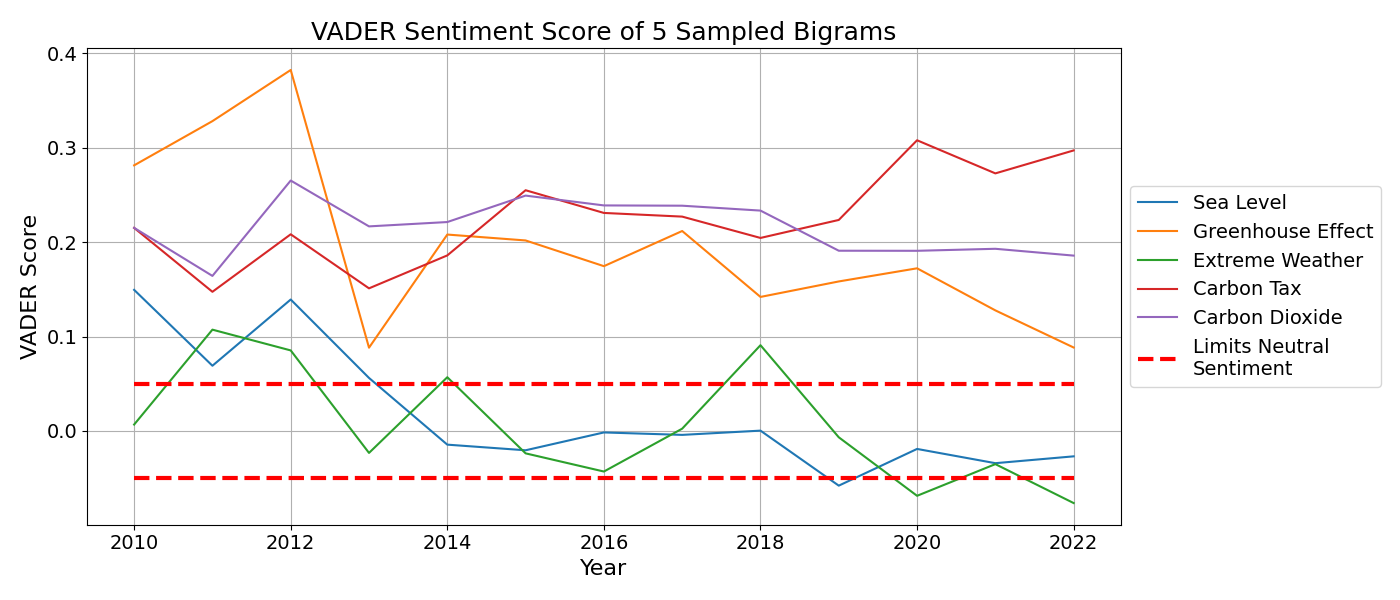
\includegraphics[width=\textwidth]{images/topic_details/ngram/sentiment_per_topic_5Bigram.png}
    \caption{Sentiment Scores of Bigrams \emph{sea level}, \emph{greenhouse effect}, \emph{extreme weather}, \emph{carbon tax} and \emph{carbon dioxide}}
    \label{fig:sentiment_bigrams}
\end{figure}
The sentiment plot in Figure \ref{fig:sentiment_bigrams} displays the VADER sentiment scores for the same set of unigrams. Sentiment scores range from -1 (very negative) to 1 (very positive), with the red dashed lines indicating the limits for neutral sentiment.

\emph{Carbon tax} shows a slight but steady increase in sentiment over the years, starting around 0.2 and rising to 0.3. This positive trend likely reflects growing support for carbon pricing as an effective way to reduce greenhouse gas emissions. The introduction of carbon taxes in various regions and their success in lowering emissions might have contributed to this positive sentiment \cite{murray2015bc}.

\emph{Greenhouse effect} reached its highest sentiment in 2012 but then dropped significantly from 0.38 to 0.09 in 2013. The peak in 2012 might be linked to increased awareness of climate change impacts and global climate agreements. However, the sharp drop in 2013 could be due to a shift in discussions towards more specific and actionable climate issues, reducing the prominence of the \emph{greenhouse effect} in public conversations \cite{ipcc2014impacts}.

\emph{Extreme weather} has fluctuating sentiments, with positive sentiment scores in 2011, 2012, 2014, and 2018. The peak in 2018 likely corresponds to heightened awareness and discussions about extreme weather events, which may have been framed positively due to increased persistence and preparedness measures. Notable extreme weather events in 2018 include a record number of wildfires in California, such as the devastating Camp Fire, which highlighted the importance of disaster preparedness and persistence \cite{CalFire2018}.
In contrast, the years 2020 and 2022 show a drop in sentiment for \emph{extreme weather} into the negative range. This shift could be attributed to the significant and devastating weather events that occurred during these years, such as the Australian bushfires (Black Summer) in 2020, which caused widespread destruction and raised global concern about climate change's impact on weather patterns \cite{BBC2020}. Additionally, the severe flooding in Pakistan in 2022 displaced millions of people and caused extensive damage, emphasizing the negative impacts of climate change on vulnerable regions \cite{cordaid2022}.

\emph{Sea level} does not show a stable sentiment over the years. It changes from positive sentiment class years (2010 - 2015) to a neutral period, with 2019 standing out with a negative sentiment class. The negative sentiment in 2019 could be linked to several alarming reports and events regarding sea level rise. For example, a report by the United Nations in 2019 highlighted the accelerated pace of sea level rise and its potential catastrophic impacts on coastal communities worldwide \cite{UN2019}.

\emph{Carbon dioxide}, on the other hand, shows a relatively stable sentiment over the years, reflecting ongoing discussions about its role in climate change without significant fluctuations in public perception.

Overall, the sentiment analysis of selected bigrams offers a detailed understanding of climate change conversations on Reddit. The positive sentiment around terms like \emph{carbon tax} suggests optimism towards policy measures for climate change mitigation. The fluctuating sentiment for \emph{extreme weather} highlights the emotional impact of these events and the varying public perceptions they generate. Similarly, the changing sentiment towards \emph{sea level} underscores the growing concern about the observable impacts of climate change on the environment.

In summary, this analysis provides valuable insights into the public's perception of different climate-related topics over time. Recognizing the positive and negative sentiments associated with these terms can help in framing climate change communication strategies to promote constructive and informed discussions.

\section{From n-grams to Entities: Enhancing Text Analysis with SpaCy}
In the previous sections, the analysis was conducted using unigrams and bigrams to identify key terms and trends in climate change discussions on Reddit. While this approach provides valuable insights, it has certain limitations. N-grams are simple sequences of words and do not account for context, variations in terminology, or the semantic relationships between terms. This is where named entity recognition (NER) using advanced natural language processing (NLP) tools like SpaCy becomes essential.

Named entities are real-world objects, such as people, organizations, locations, and events, that can be identified and categorized in text. Using SpaCy, a powerful and efficient NLP library, allows for a more sophisticated analysis by detecting these entities within the text. Here are several reasons why moving from bare n-grams to entities is advantageous:

\begin{enumerate}
    \item \textbf{Contextual Understanding:} Entities provide context that n-grams often lack. For example, the unigram \emph{Trump} could refer to different contexts depending on the discussion. By recognizing \emph{Donald Trump} as an entity, the analysis can focus specifically on mentions of the person rather than the word "Trump" in other contexts.
    \item \textbf{Normalization of Variations:} NER helps in normalizing variations of the same entity. Different ways of referring to the same entity (e.g., "U.S.A.", "United States", "America") can be identified and consolidated into a single entity, improving the accuracy and clarity of the analysis.
    \item \textbf{Reduced Noise:} N-grams often include common words that do not carry significant meaning on their own (e.g., "http", "know", "like"). Entity recognition filters out such noise by focusing on specific, meaningful entities, leading to a more focused and relevant analysis.
    \item \textbf{Sentiment Analysis:} By associating sentiments with entities rather than standalone words or phrases, the sentiment analysis becomes more accurate. For instance, analyzing the sentiment towards \emph{climate change} as an entity is more informative than analyzing the sentiment of the individual words "climate" and "change".
    \item \textbf{Enhanced Trend Detection:} Entities allow for tracking more meaningful trends over time. For instance, tracking the mentions and sentiment of specific organizations like \emph{Greenpeace} or events like \emph{Paris Agreement} provides deeper insights into public discourse and shifts in opinion.
    \item \textbf{Interconnected Insights:} Entities can be linked to other entities, providing insights into relationships and co-occurrences within the text. For example, analyzing how often \emph{climate change} is mentioned alongside \emph{renewable energy} can reveal interconnected discussions and thematic linkages.
\end{enumerate}

Making use of SpaCy and its entity recognition capabilities into the analysis allows for a richer, more detailed understanding of the discussions around climate change on Reddit. This transition from basic n-gram analysis to entity-based analysis marks a significant improvement in extracting valuable insights and making data-driven conclusions.

\section{SpaCy's Named Entities and their Frequency \& Sentiment}
In this section, the analysis moves from simple n-gram counting to a more advanced entity recognition approach using spaCy's Entity Recognizer. This method allows for a deeper understanding of the entities mentioned in climate change discussions on Reddit and their interconnections. The focus is on the entities labeled as PERSON, GPE (Geopolitical Entity), ORG (Organization), NORP (Nationalities or Religious or Political Groups), LOC (Location), and EVENT. SpaCy's entity recognition forms the basis of our analysis. Some entities have been normalized by their text (\emph{Trump} becomes \emph{Donald Trump}) or corrected by their label, while entities that were not recognized were not modified.

\subsection{An Example of Entities and their Interconnections}
Before exploring the network analysis, it is helpful to understand how entities are identified and categorized within the comments. The provided example in Figure \ref{fig:displacy} is a snippet of a Reddit comment from 2017, which has one of the lowest sentiments. This snippet displays the output of spaCy's named entity recognition (NER) tool and its visualization retrieved by displaCy, highlighting various entities within the text.

Entities are labeled as follows:
\begin{itemize}
    \item \textbf{PERSON:} Individuals mentioned, such as \emph{Sarkeesian}, \emph{Trump}, and \emph{Clinton}.
    \item \textbf{NORP:} Nationalities, religious, or political groups, such as \emph{Arab-American}, \emph{American}, and \emph{Muslim}.
\end{itemize}

\begin{figure}[h]
    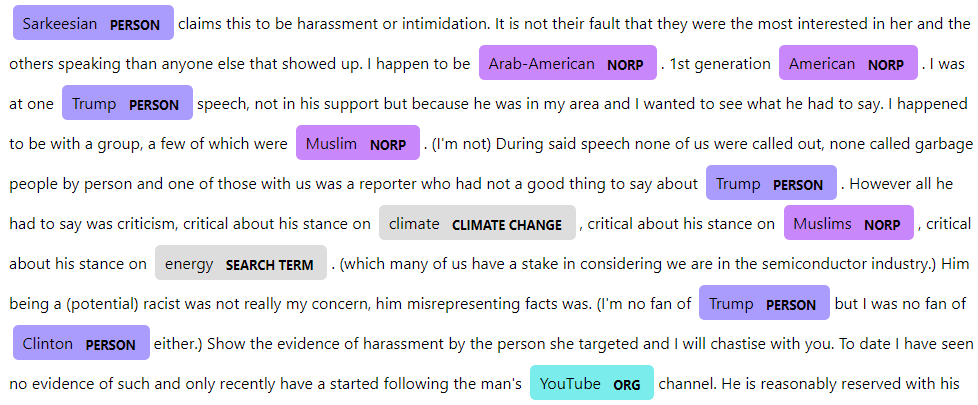
\includegraphics[width=\textwidth]{images/topic_details/entities/displaCy.PNG}
    \caption{Snippet of a Reddit Comment from 2017 with Entities Identified by SpaCy and Entity Label Corrections, Featuring the Unigram and Search Term \emph{energy}\protect\footnotemark}
    \label{fig:displacy}
\end{figure}
\footnotetext{\emph{Trump} was labeled as ORG by spaCy.}
Additionally, specific terms relevant to our analysis, like \emph{climate change} and \emph{energy}, are customized and highlighted in gray to emphasize their significance for this snippet.

Examining the interconnections within this snippet:
\begin{itemize}
    \item \emph{Sarkeesian} (PERSON) and \emph{Trump} (PERSON) are both prominent figures whose actions and statements can significantly influence public opinion. The mention of Trump is connected to a speech, which is noted for its critical stance.
    \item \emph{Arab-American} (NORP) and \emph{Muslim} (NORP) reflect the identities of individuals in the context of Trump's (PERSON) speech, highlighting the intersection of climate discourse with social and political identities.
    \item \emph{American} (NORP) is used to describe a broader national identity, often linked to discussions about national policies and leadership.
    \item \emph{Clinton} (PERSON) appears in contrast to \emph{Trump} (PERSON), showing the political divide and differences in stances on climate issues.
\end{itemize}

This method of entity recognition allows for a more structured analysis of text data, providing insights into how different entities are interconnected and discussed over time. It sets the stage for our detailed examination of network graphs, where the relationships and sentiments associated with these entities will be explored to understand the broader narrative and sentiment trends in climate change discussions.

\subsection{Network Analysis}
To visualize the relationships between these entities, network graphs have been created for each year. These graphs not only show the connections between entities but also indicate the average sentiment score associated with each entity. The sentiment scores, ranging from -1 (very negative) to 1 (very positive), are averaged from the sentiments of the comments in which the entities are mentioned.

It is important to note that many of the entities identified in these discussions are not directly related to major climate change topics. Instead, they highlight the heavy intersection between climate change and global politics. This emphasizes that climate change is not an isolated topic; it intersects with almost all major global issues today. Analyzing climate change discourse without considering the geopolitical context would provide an incomplete picture.

The decision to focus on election years for this analysis is driven by the significant impact that political leadership and election effects have on climate change policies and discourse. Election years often bring heightened attention to political figures, policies, and national priorities, making them critical periods for understanding shifts in public sentiment and discussion topics. Political campaigns, debates, and media coverage during these times can greatly influence public opinion and the prioritization of climate change in the national agenda. By examining the network of entities during election years, we can gain insights into how political dynamics shape climate change discourse and identify key influencers and sentiments that drive public conversations.

\subsubsection{2012 Network Analysis}
\begin{figure}[h]
    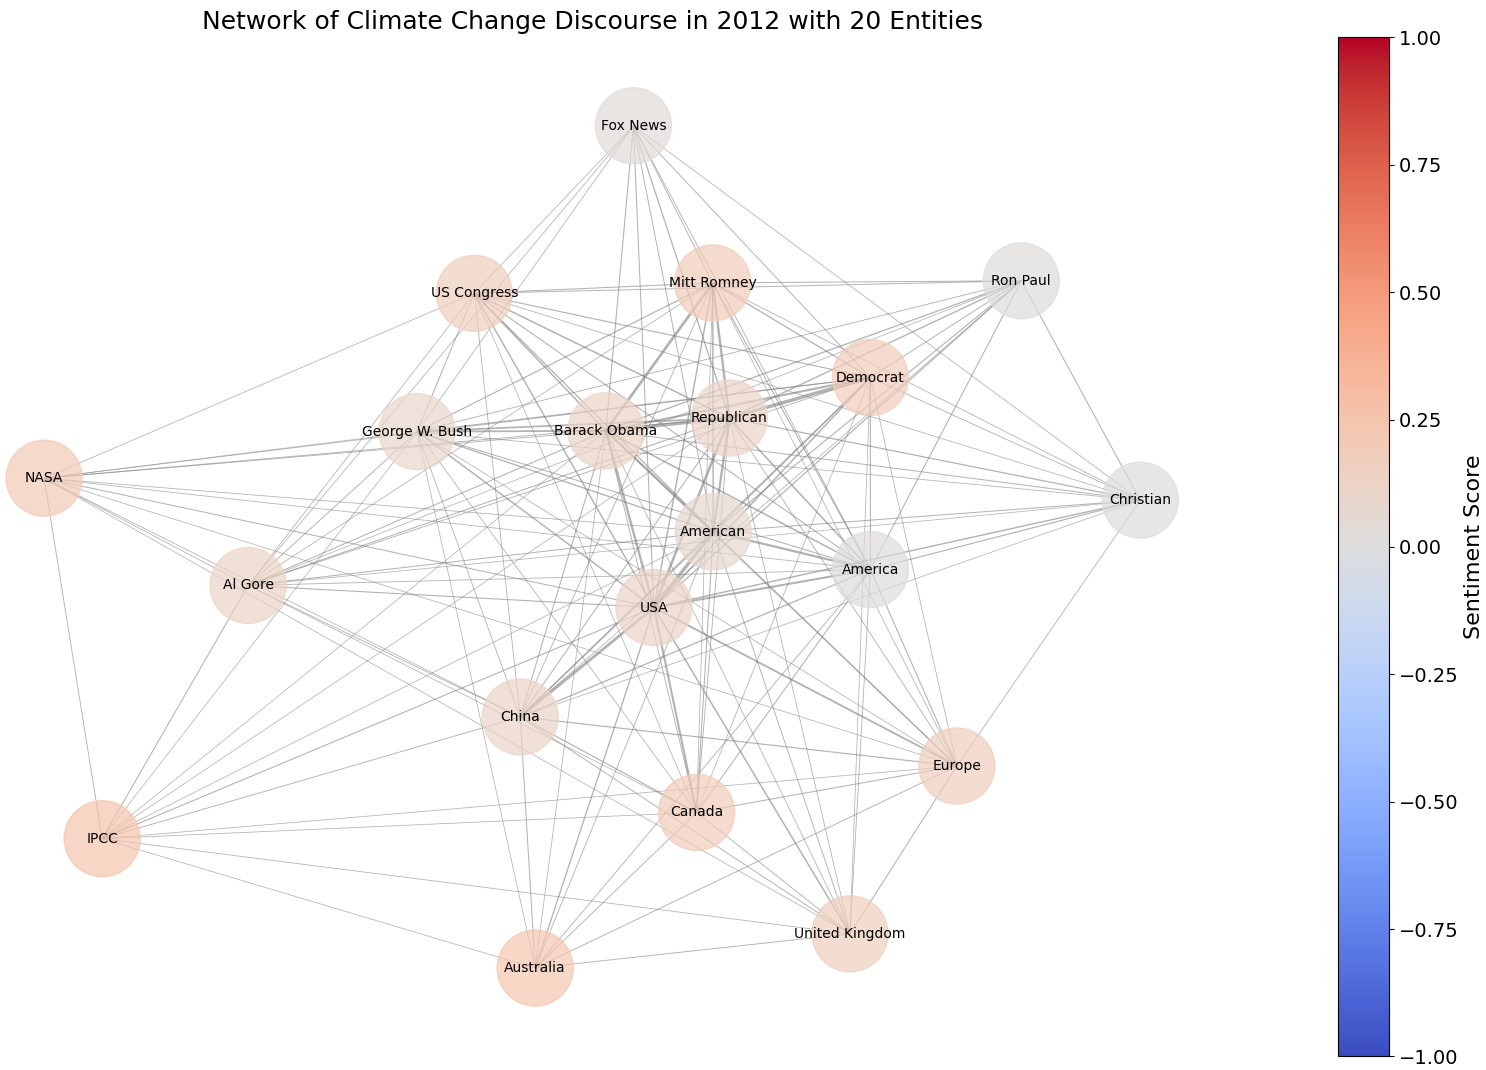
\includegraphics[width=\textwidth]{images/topic_details/entities/network_analysis_top20_2012_spring.png}
    \caption{Network of 20 Most Frequent Entities and their Sentiment in 2012}
    \label{fig:network_2012}
\end{figure}
The network graph for 2012 in Figure \ref{fig:network_2012} highlights a US-centric discourse around climate change. Key entities include political figures like Barack Obama and George W. Bush, organizations such as the US Congress and NASA, and geopolitical entities like the USA and China. The sentiment scores are predominantly neutral to slightly positive, reflecting a period of political stability and ongoing environmental initiatives.

\begin{description}
    \item[Overall Sentiment:] The 2012 graph shows the highest overall sentiment among the years analyzed, which is also visible in Figure \ref{fig:mean_sentiment}. This could be attributed to the general optimism surrounding Obama's re-election campaign, which emphasized clean energy and environmental protection \cite{obama2013climate}.
    \item[Democratic and Republican Candidates:] The key figures in the election were \emph{Barack Obama} (Democrat) and \emph{Mitt Romney} (Republican), with Obama winning re-election.
    \item[IPCC Inclusion:] The Intergovernmental Panel on Climate Change (\emph{IPCC}) is included due to its influential role in climate science and policy. The release of its assessment reports often drives significant discourse on climate change \cite{IPCC2014}. For example, the IPCC's Fourth Assessment Report, released in 2007, and the Special Report on Renewable Energy Sources and Climate Change Mitigation, released in 2011, were significant in shaping global climate policy.
    \item[Christian Entity:] The mention of \emph{Christian} with the lowest sentiment (still within the neutral sentiment class) could reflect discussions around the intersection of religion and climate change, possibly touching on topics like environmental leadership or skepticism about climate science within some religious communities. Prominent Christian figures or groups during the 2012 election year, such as Evangelical leaders and organizations like the Evangelical Environmental Network, often engage in debates on climate change from a religious perspective \cite{Veldman2019}.
\end{description}

\subsubsection{2016 Network Analysis}
\begin{figure}[h]
    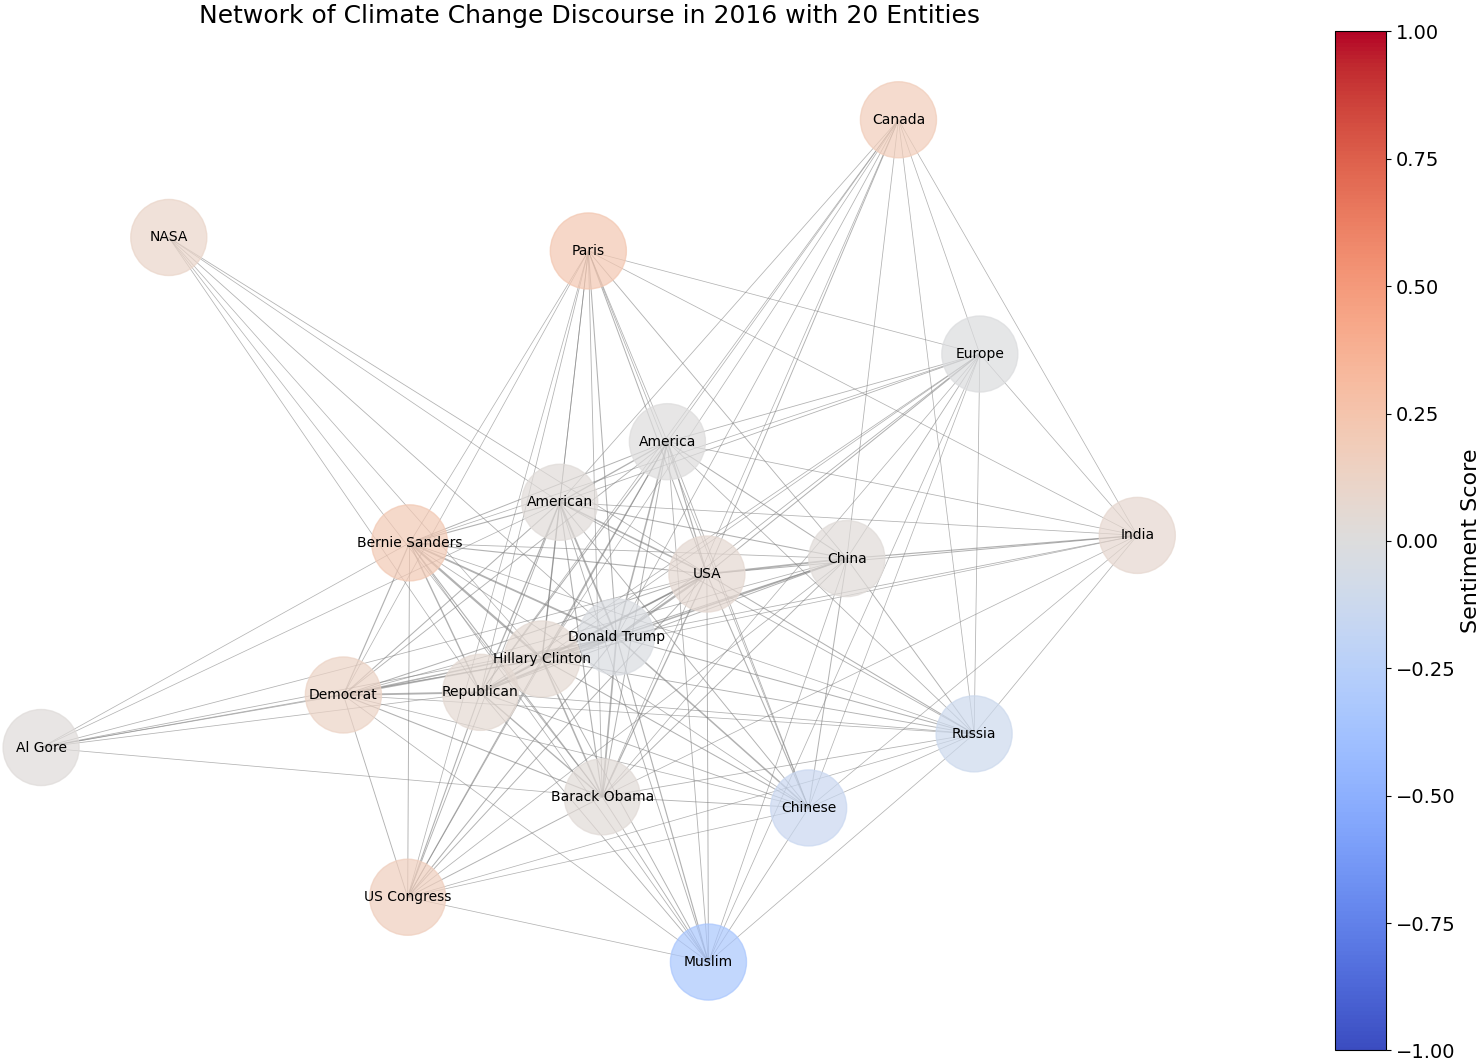
\includegraphics[width=\textwidth]{images/topic_details/entities/network_analysis_top20_2016_spring.png}
    \caption{Network of 20 Most Frequent Entities and their Sentiment in 2016}
    \label{fig:network_2016}
\end{figure}
In 2016, the network (Figure \ref{fig:network_2016}) shows a significant shift due to the US presidential election. Entities like Donald Trump, Hillary Clinton, and Bernie Sanders dominate the discourse, alongside traditional entities like the US Congress and NASA. The sentiment analysis reveals a mix of positive and negative sentiments, particularly around the election candidates, indicating polarized opinions.

\begin{description}
    \item[Democratic and Republican Candidates:] The main political figures were \emph{Donald Trump} (Republican) and \emph{Hillary Clinton} (Democrat), with Donald Trump ultimately winning the presidency despite having a lower sentiment score than Hillary Clinton. This difference may reflect the disputable nature of the election and the polarizing views on Trump's climate policies. Trump's rhetoric often focused on economic concerns over environmental regulations, which resonated with a significant portion of the voters despite generating negative sentiment in climate change discussions \cite{bbc2016trump}.
    \item[Paris Agreement:] The inclusion of \emph{Paris} is linked to the Paris Agreement, a major international treaty on climate change adopted in 2015. This agreement aimed to limit global warming and was a significant topic in climate discussions \cite{UN2019}.
    \item[Muslim Entity:] The very negative sentiment around \emph{Muslim} likely stems from the political rhetoric and policies of the time, including Trump's proposed travel ban and broader discussions around immigration and security. Trump's campaign included significant anti-immigration rhetoric, particularly targeting Muslim-majority countries, which contributed to the negative sentiment \cite{Gottfried_2023}.
    \item[Russia and Chinese Entities:] The negative sentiment around \emph{Russia} and  \emph{Chinese} could be related to discussions on international politics, cybersecurity concerns, and trade issues, all of which were prominent in 2016. Russia, often viewed negatively due to its geopolitical actions, including involvement in the Syrian Civil War and claims of interference in the US elections, likely contributed to this sentiment. The long-standing historical tensions from the Cold War also play a role in Russia's negative sentiment \cite{Ziegler2018}. For China, Trump's campaign rhetoric frequently criticized China's trade practices and accused China of currency manipulation, which fueled negative sentiments. These trade tensions and accusations of environmental irresponsibility by China in global forums added to the negative perception \cite{Steinbock2018}.
\end{description}

\subsubsection{2020 Network Analysis}
\begin{figure}[h]
    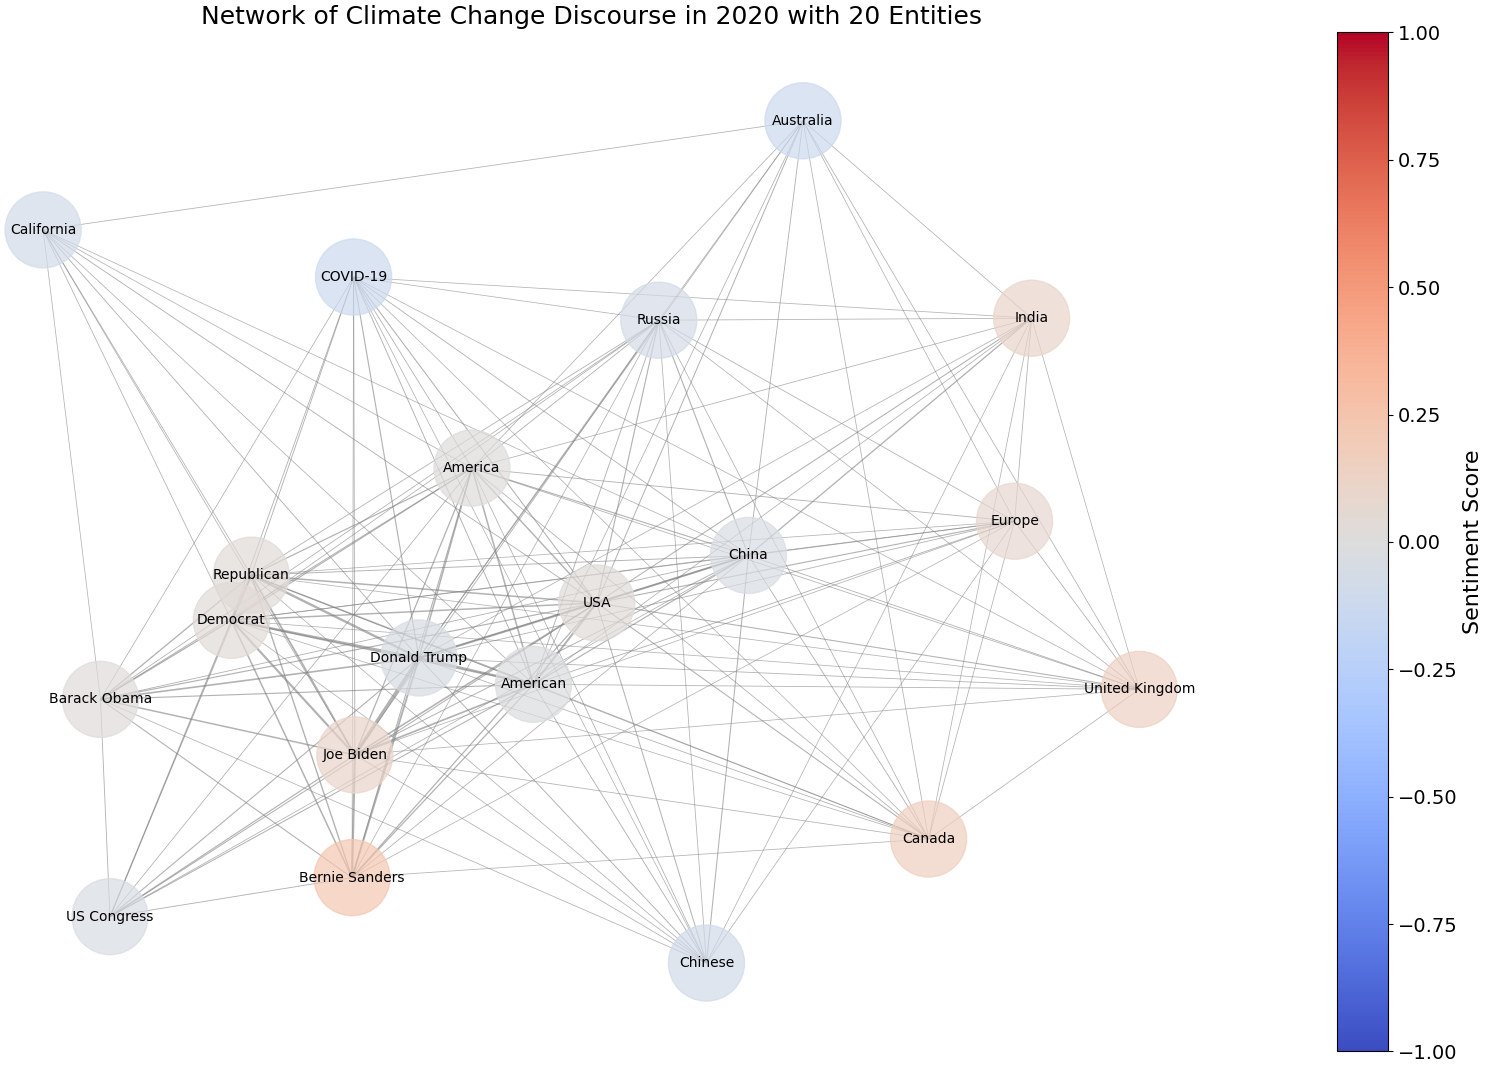
\includegraphics[width=\textwidth]{images/topic_details/entities/network_analysis_top20_2020_spring.png}
    \caption{Network of 20 Most Frequent Entities and their Sentiment in 2020}
    \label{fig:network_2020}
\end{figure}
The 2020 network graph presented in Figure \ref{fig:network_2020} is heavily influenced by the COVID-19 pandemic, with entities like \emph{COVID-19} and \emph{California} becoming prominent. The sentiment scores are more varied, reflecting the complex and diverse discussions around climate change during the pandemic. Political figures such as Donald Trump and Joe Biden are central, highlighting the impact of the US presidential election on climate change discourse.

\begin{description}
    \item[Democratic and Republican Candidates:] The key political figures in the 2020 election were \emph{Donald Trump} (Republican) and \emph{Joe Biden} (Democrat), with Joe Biden winning the presidency.
    \item[COVID-19 Pandemic:] The presence of \emph{COVID-19} reflects its global impact on all aspects of life, including environmental and climate policies. The pandemic led to discussions on how to build back better with greener policies. The significant reduction in industrial activity and transportation during the pandemic resulted in temporary decreases in carbon emissions and improved air quality in many regions. This situation highlighted the potential benefits of reducing emissions and stimulated conversations about sustainable recovery plans that integrate climate goals into economic recovery strategies \cite{JABAREEN2013220}. For instance, the water in Venice became clearer, and fish returned due to reduced boat traffic and pollution. Additionally, smog in some cities in China was significantly reduced, improving sight distance and air quality \cite{Xu_2020}. Moreover, the pandemic underscored the interconnections of global health and environmental sustainability, emphasizing the need for resilient and adaptive climate policies in the face of future crises \cite{interdisciplinary2021}.
    \item[Negative Sentiments:] Entities like \emph{Australia}, \emph{California}, \emph{Chinese}, and \emph{Russia} show negative sentiments similar to \emph{COVID-19}. This could be due to climate disasters like the Australian bushfires and California wildfires, as well as geopolitical tensions involving China and Russia. The rising conflict between Russia and Ukraine, which began escalating in 2014 and continued to burden international relations, also contributed to the negative sentiment towards Russia \cite{crisisgroup2022donbas}. Conflicts with China included trade wars initiated by Trump's administration, which heightened negative perceptions \cite{doi:10.1177/17480485231206364}.
    \item[Bernie Sanders and Canada:] \emph{Bernie Sanders} has the most positive sentiment, followed by \emph{Canada}. Sanders' progressive climate policies likely contributed to his positive sentiment. His proposals included the Green New Deal, which aimed to transition the US to 100\% renewable energy and create millions of jobs in the process \cite{sanders2020green}. Canada's environmental initiatives, such as carbon pricing, investment in green technology, and strong commitments to the Paris Agreement, have also obtained positive sentiment \cite{canada2020climate}.
\end{description}

The network analysis of climate change discourse on Reddit reveals a complex interplay of political, scientific, and global entities. The sentiment scores add a layer of understanding to how these entities are perceived, highlighting the importance of both political leadership and scientific expertise in the public discourse on climate change. This approach, using entity recognition and sentiment analysis, provides a more differentiated view of climate change discussions compared to simple n-gram analysis.

\section{Analysis of Organizational Mentions and Industrial Companies}
The analysis of frequently mentioned organizations in climate change discussions on Reddit reveals several notable trends and entities. The bar plot for 2013 (Figure \ref{fig:org_2013}) presents the frequency (absolute values are provided within the bar) and sentiment of the 15 most mentioned organizations, highlighting a strong U.S.-centric focus influenced by political and industrial contexts. This example provides an overview that helps move to analyzing the sentiment and frequency of specific U.S. companies over a broader time frame.

\begin{figure}[h]
    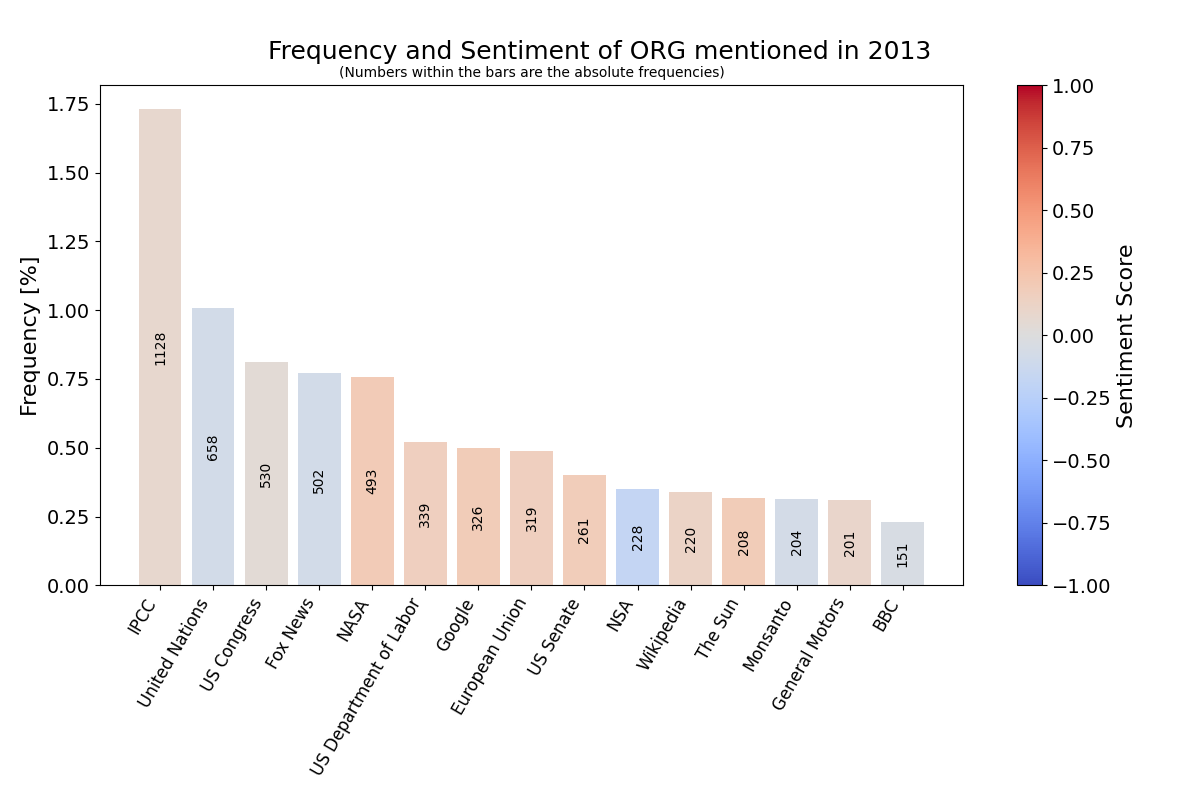
\includegraphics[width=\textwidth]{images/topic_details/entities/ORG_2013.png}
    \caption{Top 15 Most Frequent ORG Entities in 2013 with their Sentiments}
    \label{fig:org_2013}
\end{figure}

\subsection{Overview of Key Organizations in 2013}
\begin{description}
    \item[IPCC (Intergovernmental Panel on Climate Change)] The IPCC is the most frequently mentioned organization, reflecting its critical role in providing scientific assessments on climate change. With 1,128 mentions, it holds a positive sentiment score, underscoring its credibility and the reliance on its reports for climate policy and advocacy discussions. The IPCC's influence in 2013 was significant, with the release of the Fifth Assessment Report (AR5), which provided comprehensive evaluations of the physical science basis of climate change, impacts, adaptation, vulnerability, and mitigation strategies \cite{ipcc2013}.
    \item[NSA (National Security Agency)] The NSA exhibits the most negative sentiment among the listed organizations. This negative perception is likely influenced by the Edward Snowden reveals in 2013, which exposed widespread monitoring practices and triggered global debates on privacy and ethics. The  information shared by Snowden had far-reaching implications, leading to discussions about government control and civil liberties, which negatively impacted the public perception of the NSA \cite{lanchester2013}.
    \item[Monsanto] The negative sentiment towards Monsanto can be attributed to the "March Against Monsanto" protests in 2013. These protests highlighted public concerns over genetically modified organisms (GMOs) and pesticide use. The widespread demonstrations reflected the growing anxiety about Monsanto's practices and their potential impact on health and the environment \cite{guardian2013}.
\end{description}

Overall, the data from 2013 emphasize the intersection of climate change discourse with significant political and social events, highlighting the
connected nature of climate change and global governance. This U.S.-centric focus is evident from the dominance of entities related to U.S. politics and industries.

This example of 2013 leads us to a broader examination of the frequency and sentiment of specific U.S. companies, such as Amazon, Google, ExxonMobil, and Tesla. Understanding the role of these industrial giants is crucial, as they significantly influence and are influenced by climate change policies and public perception. Analyzing these companies helps to highlight the important connection between industrial activities and climate change discussions, revealing how public sentiment towards these corporations evolves over time. Industrial companies are generally important to understand, influence, and discuss climate change discourses due to their significant environmental impacts and roles in shaping sustainability practices.

\subsection{Analysis of Key U.S. Companies}
\subsubsection{Amazon}
\begin{figure}[h]
    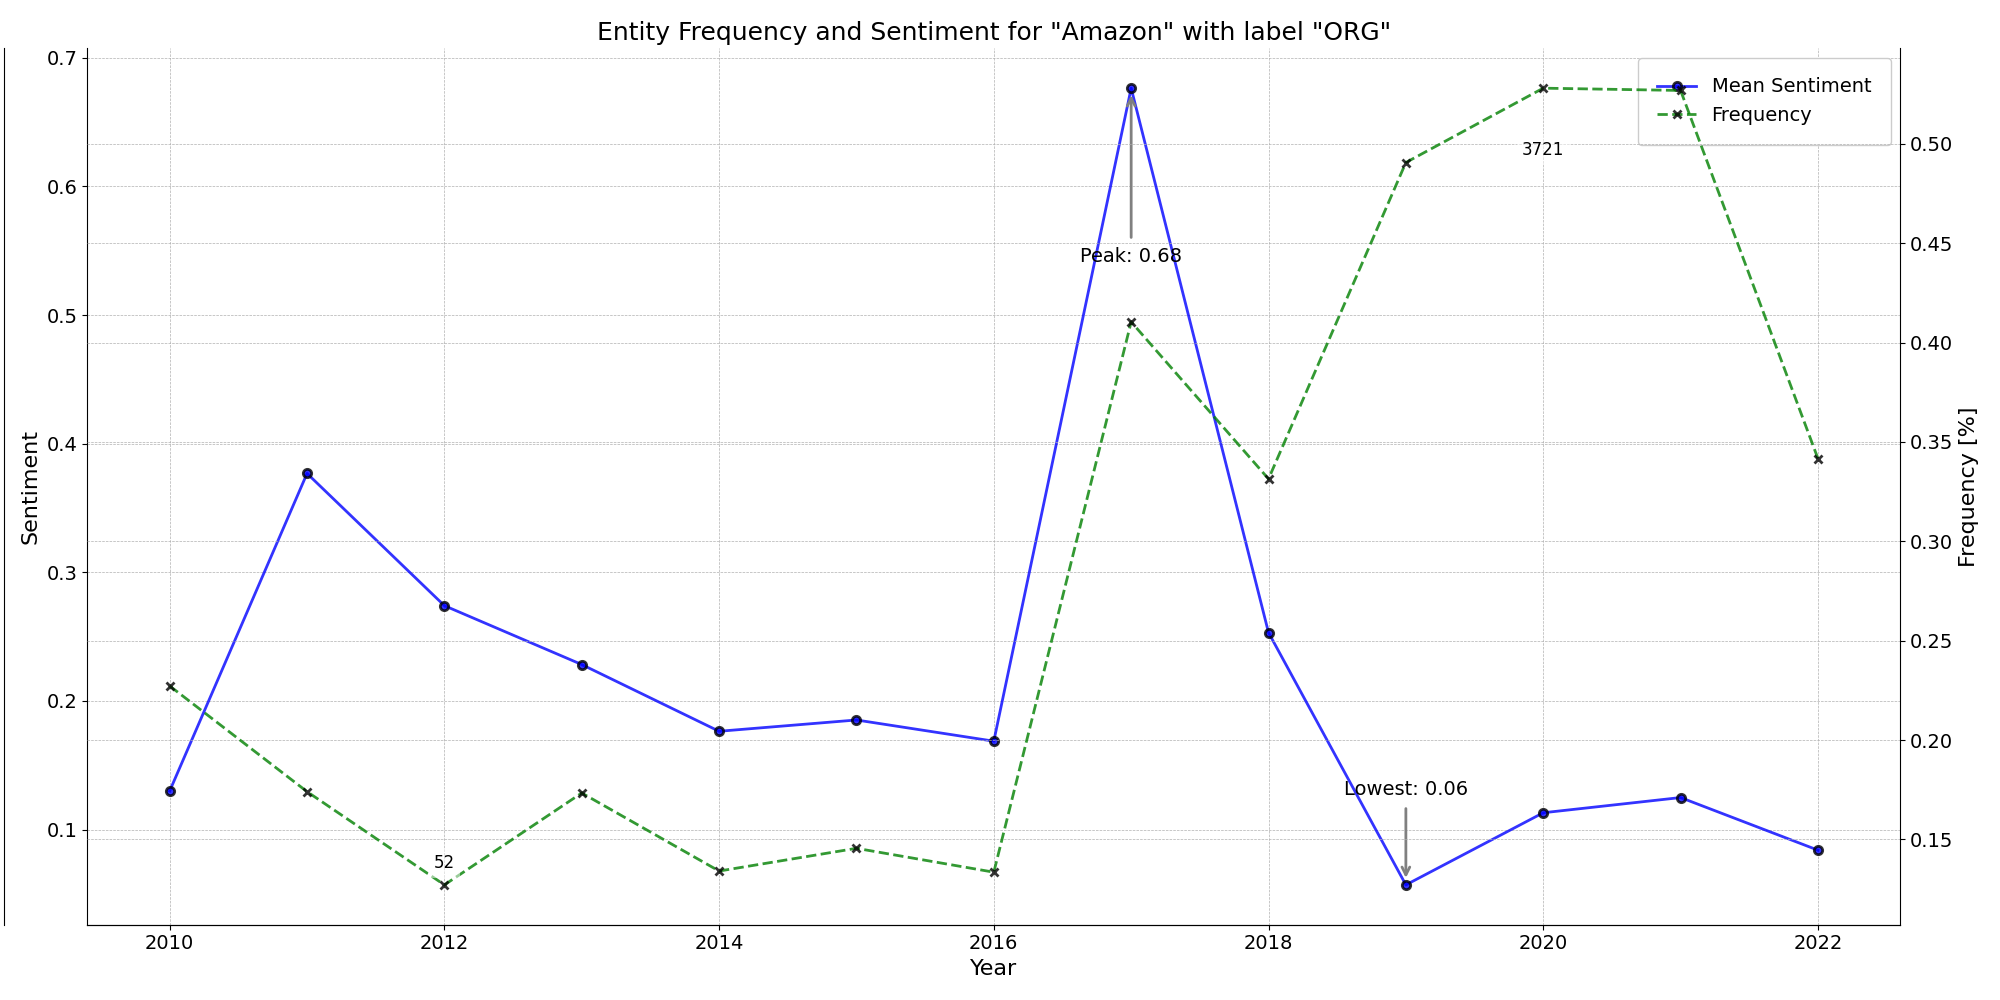
\includegraphics[width=\textwidth]{images/topic_details/entities/entity_frequency_Amazon.png}
    \caption{Trends in Amazon's Frequency and Sentiment in the Reddit Dataset}
    \label{fig:entity_amazon}
\end{figure}

Amazon is an American multinational technology company known for its e-commerce platform, cloud computing services, digital streaming, and artificial intelligence. Founded by Jeff Bezos in 1994, Amazon started as an online bookstore and quickly expanded into various other product categories. It is now one of the largest online retailers globally. The company also provides cloud computing services through Amazon Web Services (AWS), which has become a major player in the industry \cite{techtarget2024}.

Amazon shows a significant peak in frequency and sentiment in 2017, with a rapid drop in sentiment to an all-time low in 2019, followed by fluctuating trends in following years.

\begin{itemize}
    \item \textbf{2017 Peak:} The peak in 2017 corresponds to Amazon's initiatives in renewable energy investments and its commitment to sustainability, which positively impacted public sentiment \cite{amazon2017,ventura2017}.
    \item \textbf{2019 Decline:} The sharp drop in sentiment in 2019 can be linked to criticisms of Amazon's environmental practices and labor conditions. Employees staged a walkout demanding better climate policies, which negatively influenced public perception \cite{seattletimes2019}.
    \item \textbf{2020 Frequency Peak:} The highest frequency in 2020 is likely due to the COVID-19 pandemic, which increased Amazon's visibility and discussions around its operations and environmental impact. The rise in e-commerce during the pandemic brought attention to Amazon's carbon footprint and sustainability efforts \cite{moorhead2021amazon}.
\end{itemize}

\subsubsection{Google}
\begin{figure}[h]
    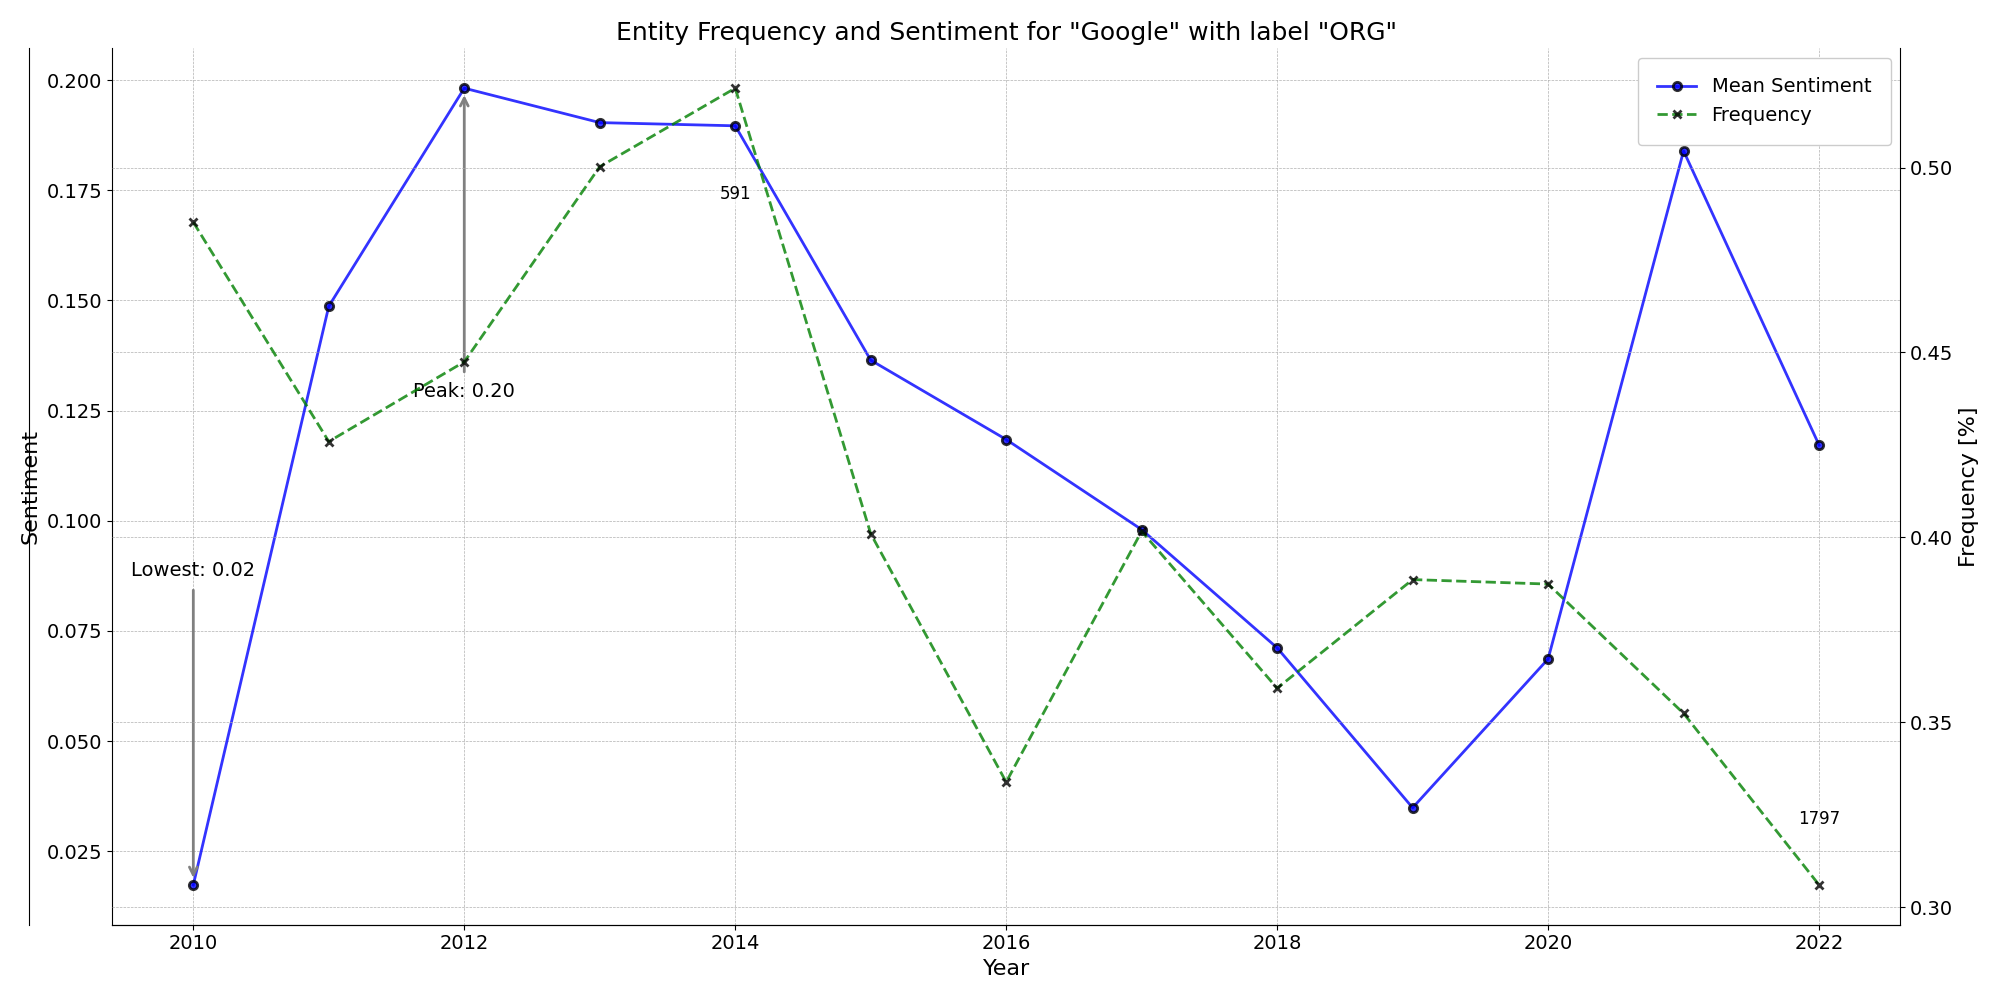
\includegraphics[width=\textwidth]{images/topic_details/entities/entity_frequency_Google.png}
    \caption{Trends in Google's Frequency and Sentiment in the Reddit Dataset}
    \label{fig:entity_google}
\end{figure}

Google, founded by Larry Page and Sergey Brin in 1998, is a leading technology company known for its search engine, advertising services, and numerous digital products such as Gmail, Google Maps, and YouTube. It operates under its parent company, Alphabet Inc., and has made significant investments in artificial intelligence, renewable energy, and autonomous driving technologies \cite{britannica2024}.

Google shows a progression from a neutral sentiment in 2010 to a peak in 2013, followed by a drop and a regrowth in 2020 and 2021.

\begin{itemize}
    \item \textbf{2012-2013 Increase:} The significant rise in sentiment during these years is due to Google's significant investments in renewable energy projects and its commitment to carbon neutrality. These efforts were well-received and highlighted Google's leadership in green technology \cite{wemeanbusiness2024,google2013}.
    \item \textbf{Subsequent Decline:} The gradual drop in sentiment might reflect growing close inspection of tech companies' environmental footprints and broader societal impacts. Issues like data privacy and corporate influence may have contributed to the mixed sentiments \cite{PENZ20181125}.
    \item \textbf{2020-2021 Resurgence:} The resurgence in positive sentiment aligns with Google's continued leadership in sustainability initiatives and advancements in green technology. Their efforts to reduce carbon emissions and promote renewable energy use have strengthened their reputation \cite{fastcompany2016}.
\end{itemize}

\subsubsection{ExxonMobile}
\begin{figure}[h]
    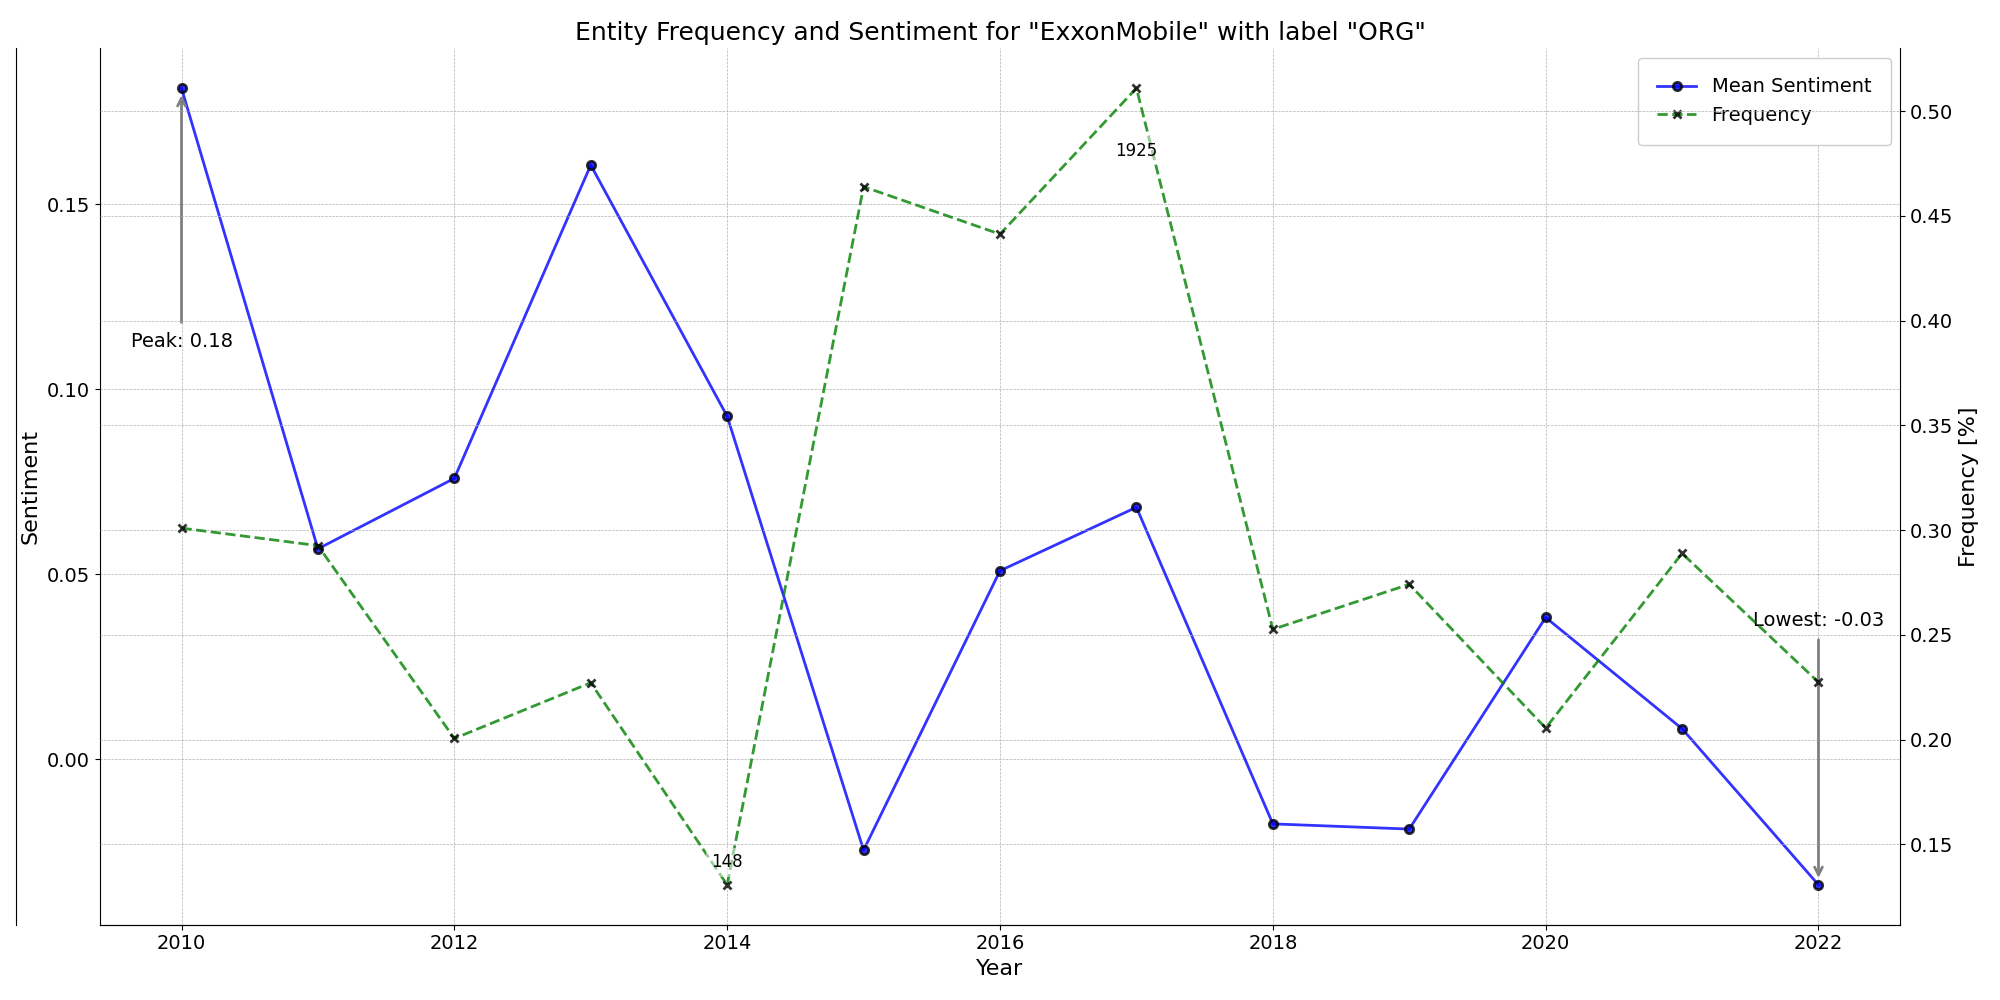
\includegraphics[width=\textwidth]{images/topic_details/entities/entity_frequency_ExxonMobile.png}
    \caption{Trends in ExxonMobil's Frequency and Sentiment in the Reddit Dataset}
    \label{fig:entity_exxonmobile}
\end{figure}

ExxonMobil is one of the world's largest publicly traded oil and gas companies, formed in 1999 through the merger of Exxon and Mobil. It is known for its widespread operations in oil exploration, production, refining, and marketing. ExxonMobil has faced criticism for its role in contributing to climate change and its historical stance on climate science \cite{worldbank2024,britannica2024exxon}.

ExxonMobil shows the highest frequencies from 2014 to 2016, with generally decreasing sentiment, nearing negative territory by 2022.

\begin{itemize}
    \item \textbf{2014-2016 High Frequencies:} These years marked intense discussions around fossil fuels and climate policies, influenced by the Obama administration's environmental regulations and global oil market dynamics. The Keystone XL pipeline debates and the Paris Agreement also played a role in increasing mentions \cite{worldbank2024,climatechangenews2015}.
    \item \textbf{2013 Sentiment Peak:} The peak in sentiment in 2013 could be attributed to ExxonMobil's public statements on reducing greenhouse gas emissions and investments in clean energy, although these claims often faced skepticism \cite{spiegel2017}.
    \item \textbf{2022 Low:} The drop to near-negative sentiment in 2022 reflects ongoing criticisms of ExxonMobil's environmental record and recognized greenwashing. Public and regulatory pressures have increased examination on fossil fuel companies \cite{plosone2024}.
\end{itemize}

\subsubsection{Tesla}
\begin{figure}[h]
    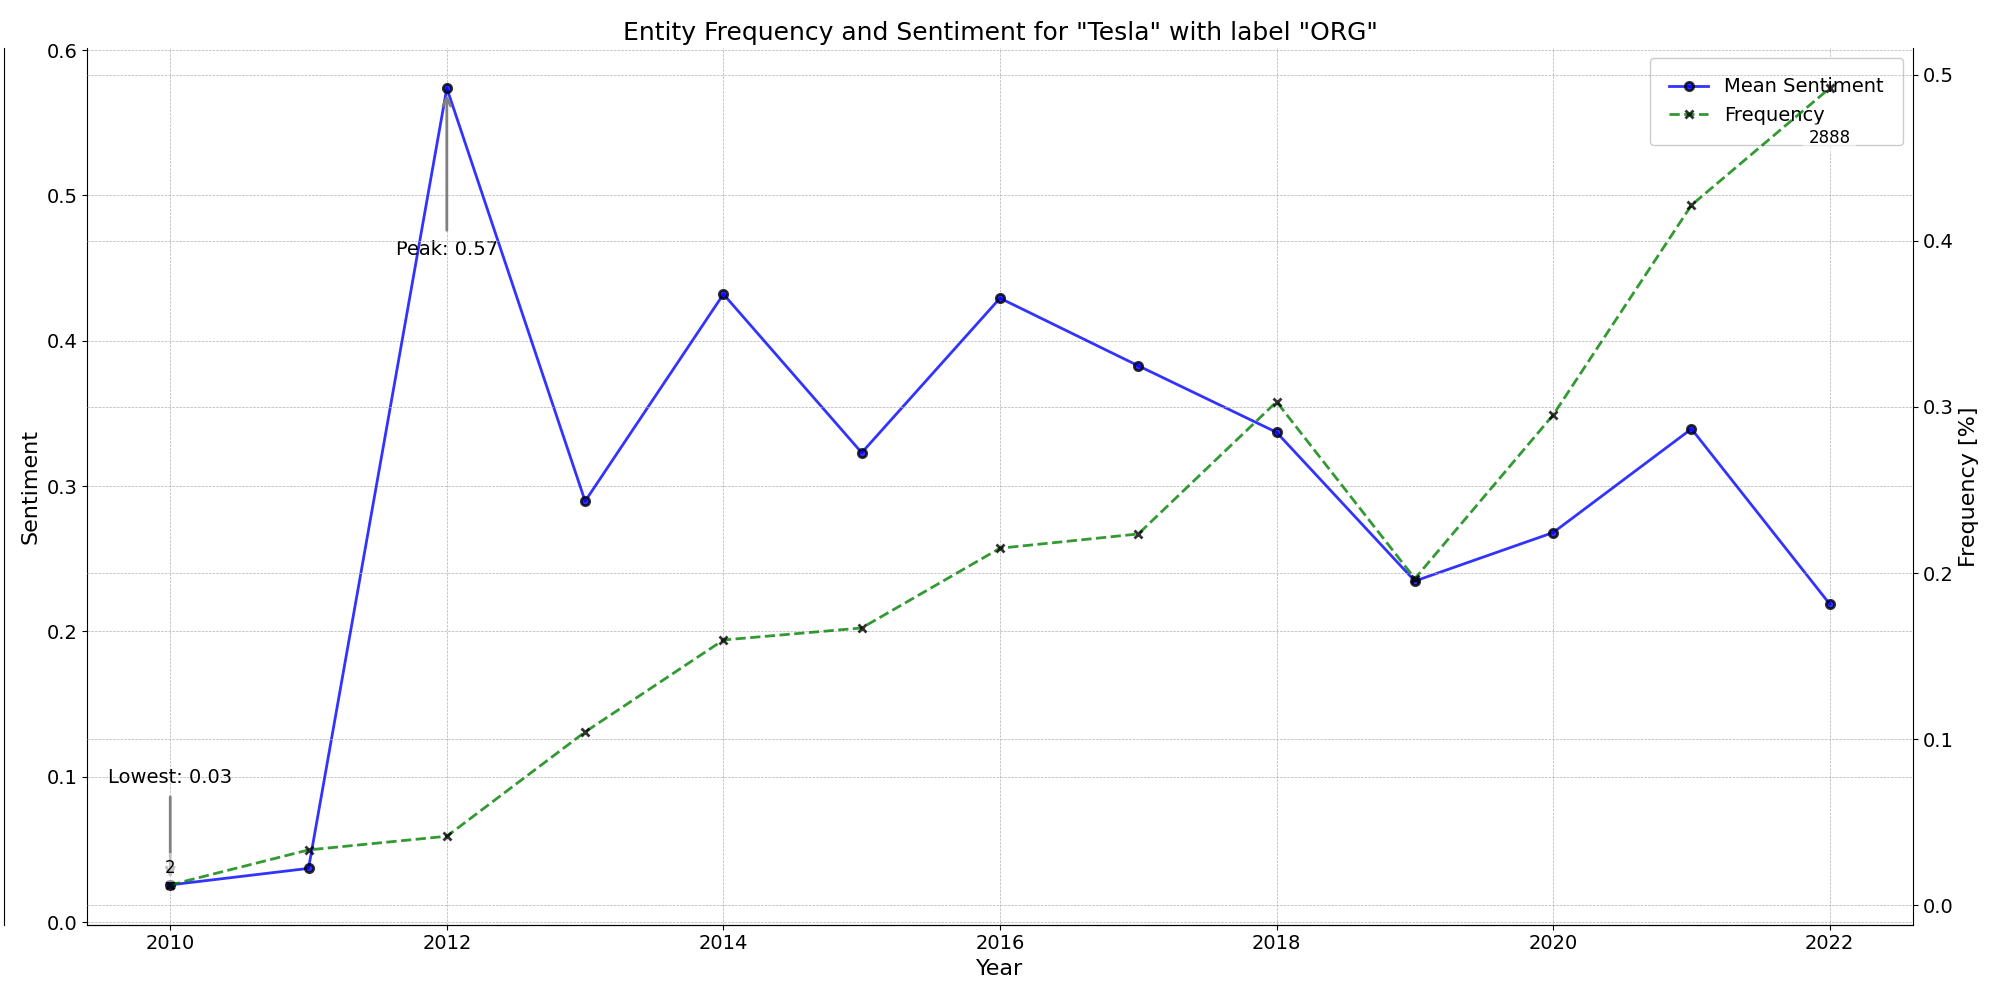
\includegraphics[width=\textwidth]{images/topic_details/entities/entity_frequency_Tesla.png}
    \caption{Trends in Tesla's Frequency and Sentiment in the Reddit Dataset}
    \label{fig:entity_tesla}
\end{figure}

Tesla, founded by Elon Musk, Martin Eberhard, Marc Tarpenning, JB Straubel, and Ian Wright in 2003, is known for its electric vehicles (EVs), energy storage solutions, and solar products. Tesla has revolutionized the automotive industry with its high-performance EVs and has been a leader in promoting sustainable energy solutions \cite{britannica2024tesla}.

Tesla exhibits a stable increase in frequency over the years, peaking in 2022. Sentiment peaked significantly in 2012, with a stable trend and slight decrease afterward.

\begin{itemize}
    \item \textbf{2012 Sentiment Peak:} The peak in sentiment in 2012 is linked to Tesla's Model S release, which revolutionized the electric vehicle market and received widespread praise. This innovation positioned Tesla as a leader in sustainable transportation \cite{tesla2012,teslamag2022}.
    \item \textbf{Stable Frequency Increase:} Tesla's frequency rise reflects its growing influence in the clean energy and automotive sectors, aligning with increased public and media attention. Tesla's innovations in battery technology and renewable energy solutions contribute to its prominence in climate change discussions.
    \item \textbf{2022 Frequency Peak:} The peak in 2022 coincides with Tesla's expanded market presence and ongoing innovations. The company's advancements in electric vehicles and energy storage solutions have kept it at the forefront of discussions about sustainable technology \cite{notateslaapp2023}.
\end{itemize}

\section{Analysis of Frequency and Sentiment of US Presidents}
\begin{figure}[h]
    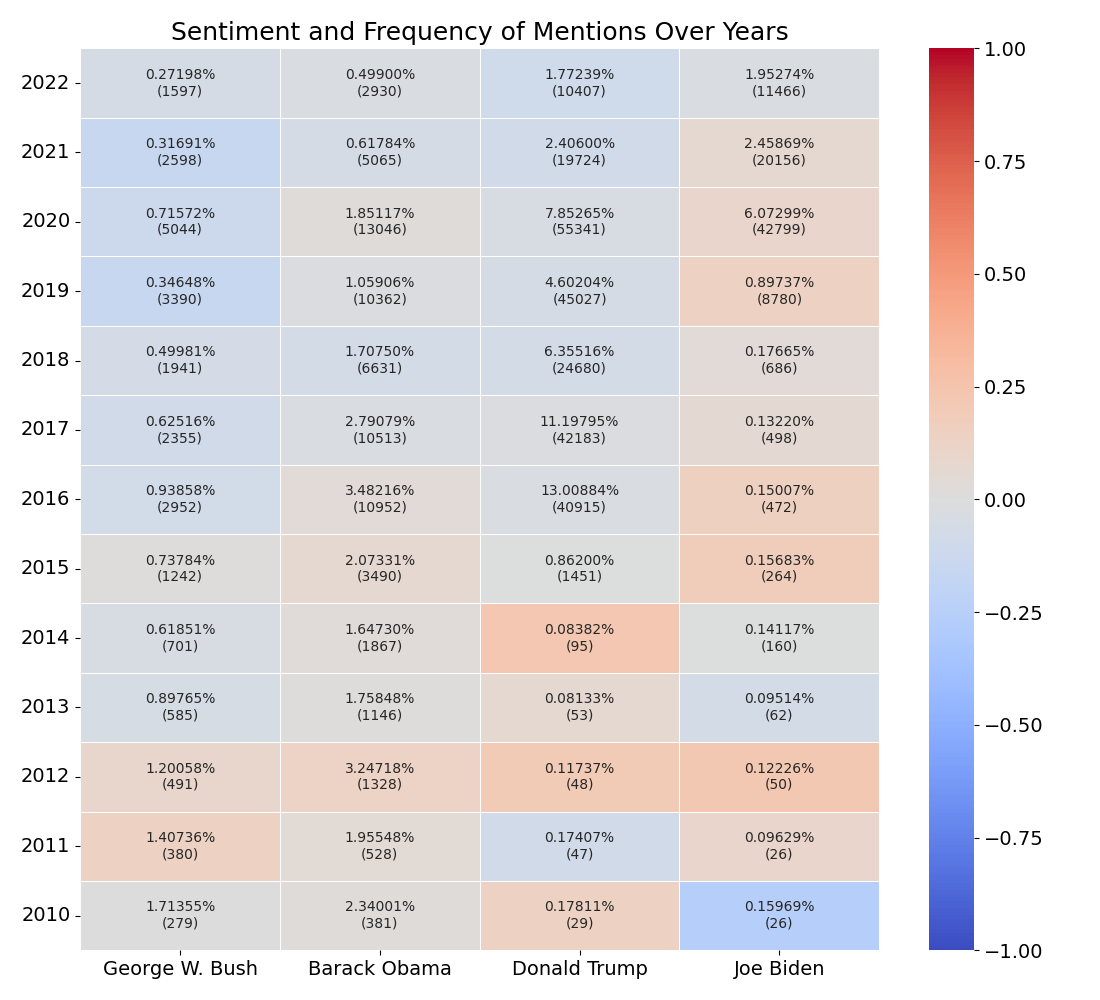
\includegraphics[width=\textwidth]{images/topic_details/entities/heatmap_sentiment_and_frequency_4entities_PERSON.png}
    \caption{Heatmap of US Presidents' Frequency and Sentiment in the Reddit Dataset}
    \label{fig:president_entities}
\end{figure}

The heatmap provided in Figure \ref{fig:president_entities} illustrates the sentiment and frequency of mentions for four US Presidents (George W. Bush, Barack Obama, Donald Trump, and Joe Biden) from 2010 to 2022. This analysis explores the patterns observed in the data, focusing on peaks and drops in both frequency and sentiment.
The dataset covers the period from 2010 to 2022 and includes mentions of four US Presidents:

\begin{itemize}
    \item \textbf{George W. Bush:} Although his presidency ended in 2009, he remains part of the discourse, particularly in relation to his climate policies \cite{Meyer2023}.
    \item \textbf{Barack Obama:} President from 2009 to 2017, with a continued presence in the climate change discussion post-presidency \cite{obamaclimatechangerecord}.
    \item \textbf{Donald Trump:} President from 2017 to 2021, who remains a significant figure in climate change discourse even after his term ended \cite{bbc2020trump}.
    \item \textbf{Joe Biden:} Elected in 2020 and currently serving as president, showing a notable presence in recent years \cite{wri2022biden}.
\end{itemize}

Election years show significant peaks in mentions for the presidents involved in the campaigns. For instance, 2016 shows a substantial increase in mentions for Donald Trump as he ran for and was elected president. Similarly, in 2020, both Donald Trump and Joe Biden show peaks in mentions due to their participation in the presidential election. These peaks highlight the heightened public and media attention during election periods.

Even after their terms, presidents maintain a presence in climate change discourse. George W. Bush continues to be mentioned, although his frequency decreases over time. Barack Obama remains consistently mentioned, reflecting ongoing discussions about his climate policies and initiatives. Donald Trump, in particular, maintains an unusually high frequency in mentions even after his presidency, especially in 2021 and 2022. This can be attributed to his polarizing climate policies, continued public statements, actions that keep him in the public eye, and his extensive use of social media to communicate with the public \cite{trumptruthsocial}. Joe Biden, as the current president, naturally has high mentions reflecting his active role in current climate policies.

George W. Bush's sentiment decreases over the years, indicating increasing skepticism toward his climate policies. This trend could be due to the long-term impacts of his administration's policies becoming more apparent over time. Barack Obama's sentiment remains relatively stable, suggesting a balanced view of his climate actions, with his efforts in the Paris Agreement and renewable energy investments being positively received. Donald Trump's sentiment shows a slight drop, reflecting controversies and criticisms surrounding his climate policies, such as exit from the Paris Agreement and promoting fossil fuels \cite{state2020,columbiaclimate2024}. However, the sentiment for Trump has notable peaks and drops, with 2014 and 2020 being outliers, likely due to fewer mentions causing fluctuation.

Joe Biden exhibits the most positive overall sentiment among the presidents during the data period. This could be attributed to his strong stance on climate change, rejoining the Paris Agreement, and ambitious climate policies like the Infrastructure Bill aimed at promoting clean energy and reducing emissions. His proactive approach and clear commitment to addressing climate issues resonate positively with the public and media.

Even after not being re-elected, Donald Trump continues to have a high frequency of mentions. This untypically high frequency is likely due to his continuous involvement in public debates, media coverage of his statements, ongoing influence within the political landscape, and his significant presence on social media platforms \cite{trumptruthsocial}. His controversial and often polarizing views on climate change ensure he remains a significant topic of discussion.

Joe Biden's positive sentiment reflects his clear and consistent climate policies, which align with scientific consensus and international efforts to fight climate change. His administration's efforts to reverse Trump's policies and reestablish environmental protections contribute to this positive perception \cite{grist2023}.

The decrease in sentiment for ex-presidents can be attributed to backdated evaluations of their policies. Once out of office, the long-term impacts of their decisions become clearer, often leading to more critical assessments. For example, George W. Bush's sentiment decline reflects ongoing skepticism about his administration's climate actions, while Donald Trump's decreasing sentiment post-presidency highlights continued debates surrounding his policies.

Overall, climate policy tends to be viewed more skeptically after a president's term ends. This backdated view allows for a more critical assessment of the effectiveness and consequences of their policies. The sentiment trends observed for George W. Bush and Donald Trump indicate that the public and media often re-evaluate the impacts of past administrations with a more critical viewpoint, leading to decreased sentiment over time.

This detailed analysis underscores the dynamic nature of public and media perception of US Presidents in the context of climate change. Election periods, ongoing public involvement, and backdated evaluations play significant roles in shaping both the frequency of mentions and the sentiment towards these leaders.

\chapter{Discussion and Conclusion}
\section{Summary of Findings}
\subsection{Data Trends and Sentiment Analysis}
The analysis began with examining the frequency and sentiment of climate change discussions on Reddit from 2010 to 2022. The increasing volume of discussions over the years, especially during significant climate events like the Fridays for Future protests and the Australian bushfires in 2019, highlighted how public interest and engagement grew sharply in response to key events. This initial analysis provided a foundation for understanding broader patterns in discourse.

Sentiment analysis revealed that, in absolute terms, there were slightly more negative comments (2,109,360) than positive comments (2,067,883). Neutral comments were significantly fewer (423,455). However, on a yearly basis, it was observed that positive sentiment often exceeded negative sentiment in most years. Specifically, from 2010 to 2017, and in 2021, positive comments were more frequent. Only in the years 2018, 2019, 2020, and 2022 did negative comments dominate positive ones. This indicates that while overall discussions had a slightly negative tone, there were significant periods where positive sentiment was more prevalent, reflecting optimism and proactive engagement. Nonetheless, the last years, particularly 2018, 2019, 2020, and 2022, were characterized by a predominance of negative sentiment, suggesting increased public concern or frustration with climate-related issues during these periods.

\subsection{Key Terms and Entities}
An analysis of specific words and phrases (unigrams and bigrams) identified key terms such as "carbon tax", "renewable energy", "sea level", and "greenhouse effect". This revealed a strong public interest in policy measures and sustainable solutions. Named Entity Recognition (NER) helped identify important organizations and political figures central to the climate change discourse, such as the United Nations.

\subsection{US Presidents and Climate Change}
Mentions of US Presidents from 2010 to 2022 provided insight into public perceptions of their climate policies. Barack Obama and Joe Biden generally received more positive sentiment, reflecting approval of their proactive climate actions. Conversely, George W. Bush and Donald Trump faced more negative sentiment, particularly post-presidency, highlighting skepticism and criticism of their climate policies. Donald Trump's untypically high frequency of mentions, even after his presidency, was attributed to his significant social media presence and polarizing views on climate change.

\section{Connecting the Findings}
The exploration began with a broad analysis of data trends and sentiment, which set the foundation for a more focused investigation into specific terms and entities. This journey brought to light the public's nuanced views on climate change policies and key figures influencing the discourse. By connecting these layers of analysis, the core research question was addressed:


\textbf{What are the patterns of public sentiment and discourse on climate change in social media, and how do they evolve over time?}
\begin{enumerate}
    \item \textbf{How does the frequency of specific unigrams and bigrams about climate change evolve over time?}
    \begin{itemize}
        \item The analysis showed that the frequency of terms like "carbon tax" and "renewable energy" increased over time, reflecting a shift in public interest towards actionable solutions. Early discussions focused on basic concepts like the "greenhouse effect", while later conversations included more specific and actionable topics such as "carbon emissions", "clean energy", and "climate policy". These shifts indicate a maturation in public engagement with climate change, moving from awareness to a focus on policy and action.
    \end{itemize} 
    \item \textbf{How does the sentiment associated with specific unigrams and bigrams about climate change evolve over time?}
    \begin{itemize}
        \item Sentiment analysis revealed a complex picture. While the overall tone of discussions had slightly more negative comments in absolute terms, many years showed a predominance of positive sentiment, particularly from 2010 to 2017 and in 2021. Negative sentiment was more dominant in 2018, 2019, 2020, and 2022. This indicates a fluctuating but generally optimistic public engagement with climate solutions during most of the period studied. Nonetheless, the last years, particularly 2018, 2019, 2020, and 2022, were characterized by a predominance of negative sentiment, suggesting increased public concern or frustration with climate-related issues during these periods.
    \end{itemize}
\end{enumerate}

\section{Integrated Discussion Points}
\subsection{The Role of Social Media and Key Events}
Social media platforms like Reddit have a significant impact on shaping public discourse on climate change. The platform allows for a diverse range of opinions and higher engagement compared to traditional media. This dynamic environment can raise both constructive discussions and polarized debates. Significant events and movements, such as the Paris Agreement and major natural disasters, heavily influence the volume and sentiment of climate discussions. These events often trigger rise in both positive and negative sentiments, reflecting the public's emotional response. For example, the Fridays for Future protests led by Greta Thunberg generated a significant increase in climate change discussions, highlighting the power of social movements in driving public discourse.

\subsection{Public Perception of Policies and Key Figures}
The analysis showed that public perception of climate policies is heavily influenced by their effectiveness and transparency. Proactive and transparent policies tend to receive positive sentiment, while regressive or harmful policies attract criticism. This is evident in the sentiment towards different US Presidents. Barack Obama and Joe Biden received positive sentiments for their proactive climate actions, while George W. Bush and Donald Trump faced negative sentiments due to skepticism and criticism of their policies. The critique of former presidents underscores the importance of sustainable and forward-thinking climate policies that can withstand long-term evaluations. As the impacts of their policies become clearer over time, public sentiment tends to become more critical, highlighting the need for policies that are both effective and adaptable to future challenges.

\subsection{Evolution of Climate Terminology and Public Engagement}
The shift in frequently used terms over time indicates that public understanding and discourse on climate change have evolved. Early discussions focused on basic concepts like the "greenhouse effect", but over time, they have shifted towards more specific and actionable topics such as "carbon tax", "renewable energy", and "sea level rise". This trend suggests that public engagement with climate issues is becoming more sophisticated and solution-oriented. As people become more informed, their discussions reflect a deeper understanding of the complexities of climate change and a greater focus on practical solutions and policies. This evolution in terminology and focus points to an increasing public awareness and readiness to support and promote for actionable climate measures.

\section{Conclusion}
This thesis demonstrates the value of using NLP techniques to analyze large-scale textual data and gain insights into public discourse on climate change. By examining discussions on Reddit, a detailed understanding of how public opinion evolves and reacts to key events and policies has been provided.

The findings emphasize the importance of proactive and transparent climate policies that align with public expectations and scientific recommendations. They also highlight the significant role of social media in shaping public discourse and the need for communicators to balance critical discussions with positive and solution-oriented narratives.

Moving forward, these insights can inform policymakers, environmental organizations, and communicators in their efforts to engage the public more effectively and encourage constructive dialogue on climate change. Future studies should explore other social media platforms and integrate more different datasets to capture a broader range of perspectives and cultural contexts.

Understanding the dynamics of public discourse on climate change is crucial for driving effective action and achieving meaningful progress in addressing this pressing global issue. This thesis contributes to that understanding by providing detailed insights into the patterns and sentiments that characterize climate change discussions on Reddit.

\chapter{Limitations and Future Work}
\subsubsection{Limitations}
Several limitations were encountered in this study, which should be considered when interpreting the findings:
\begin{description}
    \item[Data Source Limitation:] The analysis relied only on Reddit data. While Reddit is a popular platform with diverse opinions, it may not fully represent the broader public discourse on climate change. Other social media platforms, news articles, and forums could provide additional perspectives and a more comprehensive understanding.
    \item[Temporal Constraints:] The dataset covers the period from 2010 to 2022. Although this period includes significant developments in climate change discourse, the analysis might miss historical context or earlier trends that could provide deeper insights into the evolution of public sentiment and discourse.
    \item[Sentiment Analysis Accuracy:] Sentiment analysis tools, while powerful, are not perfect. They can misinterpret sarcasm, irony, or context-specific language, leading to potential inaccuracies in sentiment classification. Additionally, the tools used may not account for the nuances of climate change terminology and discussions \cite{liu2012}.
    \item[NER Limitations:] The current Named Entity Recognition (NER) implementation included entity text normalization (e.g., "obama" to "Barack Obama" and "Barack Obama" to "Barack Obama") on a lexicon-based level. Most obvious labels were corrected (e.g., "Trump" was recognized as ORG and corrected to PERSON). However, since this approach is lexicon-based, many incorrect entities remain, and it only covers detected entities. There are likely many occurrences that were not detected at all.
    \item[Language and Regional Bias:] The analysis focused on English-language comments, potentially overlooking significant contributions in other languages. Furthermore, the dataset is US-centric, missing perspectives from other continents. Including data from regions like China (e.g., Weibo) could enhance data quality and allow for analysis of regional differences in events and discourse \cite{8554131}.
    \item[Static Analytical Models:] The analytical models used in this study are static and may not adapt well to evolving language and discourse patterns. Continuous updates and improvements of these models are necessary to maintain accuracy over time.
\end{description}

\subsubsection{Future Work}
Building on the findings and addressing the limitations, several possibilities for future research are suggested:
\begin{description}
    \item[Incorporating Diverse Data Sources:] Future studies should integrate data from multiple social media platforms (e.g., Twitter, Facebook), news websites, and forums to capture a more complete overview of public discourse on climate change. This would help mitigate platform-specific biases and provide a richer dataset.
    \item[Extending Temporal Coverage:] Expanding the dataset to include earlier periods could offer valuable historical context and reveal longer-term trends in climate change discourse. This would help in understanding how public sentiment and discussion topics have evolved over decades.
    \item[Enhancing Sentiment Analysis Techniques:] Employing more advanced sentiment analysis techniques, such as deep learning models and context-aware algorithms, could improve the accuracy of sentiment classification. Integrating domain-specific lexicons and training models on climate-related texts can also improve performance \cite{liu2012}.
    \item[Improving Entity Recognition:] Improving NER models to better capture climate-related entities and integrating manual validation steps can improve the accuracy and completeness of entity recognition. Future work could also explore the relationships between entities to provide deeper insights into the discourse network. Advanced methods like contextualized embeddings (e.g., BERT) could be used to improve entity recognition \cite{Devlin2019BERTPO}
    \item[Language and Regional Bias:] Expanding the analysis to include comments in multiple languages and considering regional variations in discourse can provide a more global perspective on climate change discussions. Cooperation with linguists and regional experts can help in adapting models to different linguistic and cultural contexts. Additionally, adding data from other regions, such as China and platforms like Weibo, can improve the dataset and provide a fuller analysis of regional differences \cite{8554131}.
    \item[Dynamic Models:] Developing dynamic models that can adapt to changing language and discourse patterns over time would improve the strength of the analysis. These models could be periodically updated with new data to keep their relevance and accuracy.
    \item[Longitudinal Studies:] Conducting longitudinal studies to track changes in public sentiment and discourse over extended periods can provide deeper insights into the factors driving these changes. This approach can help in identifying long-term trends and the impact of major events on public opinion.
    \item[Policy Impact Analysis:] Future research could focus on analyzing the impact of specific climate policies and initiatives on public sentiment and discourse. This would involve correlating policy changes with shifts in sentiment and discussion topics to assess their effectiveness and public reception.
\end{description}

By addressing these limitations and exploring these paths for future research, a broader and deep understanding of public discourse on climate change can be achieved, eventually contributing to more effective communication and policy-making in this critical area.


%Beispielliteratur
\newpage
\bibliography{references}
\bibliographystyle{acl_natbib}

\newpage

% Abbildungsverzeichnis (kann auch nach dem Inhaltsverzeichnis kommen)
\listoffigures
\newpage

% Tabellenverzeichnis (kann auch nach dem Inhaltsverzeichnis kommen)
\listoftables
\newpage

\addchap{Contents of the enclosed software/data package}
All Python code, LaTeX files, and PDFs related to this study will be available on GitHub at the following repository: 

\vspace{1em}

\url{https://github.com/nurzatdzholchubekova/BachelorsThesisNDzholchubekovaLMU2024}. 

\vspace{1em}

This repository will include all necessary scripts and resources to reproduce the analyses and figures presented in this thesis.

\end{document}